\documentclass[letterpaper]{article}
\usepackage[margin=1.0in]{geometry}
\usepackage{authblk}
\usepackage{amsmath, amssymb, amsthm, mathtools}
\usepackage{graphicx}
\usepackage{caption}
\usepackage{color}
\usepackage{subcaption}

\def\btau{\boldsymbol\tau}
\def\bsigma{\boldsymbol\sigma}
\def\bbeta{\boldsymbol\beta}
\def\blambda{\boldsymbol\lambda}

\newcommand{\bs}[1]{\boldsymbol{#1}}
\DeclareMathOperator{\diag}{diag}
\DeclareMathOperator*{\argmin}{\arg\,\min}

\newcommand{\equaldef}{\stackrel{\mathrm{def}}{=}}

\newcommand{\tablab}[1]{\label{tab:#1}}
\newcommand{\tabref}[1]{Table~\ref{tab:#1}}

\newcommand{\theolab}[1]{\label{theo:#1}}
\newcommand{\theoref}[1]{\ref{theo:#1}}
\newcommand{\eqnlab}[1]{\label{eq:#1}}
\newcommand{\eqnref}[1]{\eqref{eq:#1}}
\newcommand{\seclab}[1]{\label{sec:#1}}
\newcommand{\secref}[1]{\ref{sec:#1}}
\newcommand{\lemlab}[1]{\label{lem:#1}}
\newcommand{\lemref}[1]{\ref{lem:#1}}

\newcommand{\mb}[1]{\mathbf{#1}}
\newcommand{\mbb}[1]{\mathbb{#1}}
\newcommand{\mc}[1]{\mathcal{#1}}
\newcommand{\norm}[1]{\left\| #1 \right\|}
\newcommand{\snorm}[1]{\left| #1 \right|}
\newcommand{\LRp}[1]{\left( #1 \right)}
\newcommand{\LRs}[1]{\left[ #1 \right]}
\newcommand{\LRa}[1]{\left\langle #1 \right\rangle}
\newcommand{\LRc}[1]{\left\{ #1 \right\}}
\newcommand{\tanbui}[2]{\textcolor{blue}{\sout{#1}} \textcolor{red}{#2}}
\newcommand{\Grad} {\ensuremath{\nabla}}
\newcommand{\Div} {\ensuremath{\nabla\cdot}}
\newcommand{\Nel} {\ensuremath{{N^\text{el}}}}
\newcommand{\jump}[1] {\ensuremath{\LRs{\![#1]\!}}}
\newcommand{\uh}{\widehat{u}}
\newcommand{\fnh}{\widehat{f}_n}
\renewcommand{\L}{L^2\LRp{\Omega}}
\newcommand{\pO}{\partial\Omega}
\newcommand{\Gh}{\Gamma_h}
\newcommand{\Gm}{\Gamma_{-}}
\newcommand{\Gp}{\Gamma_{+}}
\newcommand{\Go}{\Gamma_0}
\newcommand{\Oh}{\Omega_h}
\newcommand{\ptl}{{\partial}}
\newcommand{\bfsig}{\mbox{\boldmath $\sigma$}}
\newcommand{\bfn}{\mbox{\boldmath $n$}}
\newcommand{\bfH}{\mbox{\boldmath $H$}}
\newcommand{\HdivK}{\bfH(\text{div},K)}
\newcommand{\HOneK}{H^{-1}(K)}
\newcommand{\HOneOmegah}{H^{-1}(\Omega_h)}
\newcommand{\HdivOmegah}{\bfH(\text{div},\Omega_h)}
\newcommand{\vdeltau}{v_{\delta\bs u_h}}
\newcommand{\taudeltau}{\btau_{\delta\bs u_h}}

\newcommand{\eval}[2][\right]{\relax
  \ifx#1\right\relax \left.\fi#2#1\rvert}

\def\etal{{\it et al.~}}

\newcommand{\vect}[1]{\ensuremath\boldsymbol{#1}}
\newcommand{\tensor}[1]{\underline{\vect{#1}}}
\newcommand{\del}{\Delta}
\newcommand{\grad}{\nabla}
\newcommand{\curl}{\grad \times}
\renewcommand{\div}{\grad \cdot}
\newcommand{\ip}[1]{\left\langle #1 \right\rangle}
\newcommand{\eip}[1]{a\left( #1 \right)}
\newcommand{\pd}[2]{\frac{\partial#1}{\partial#2}}
\newcommand{\pdd}[2]{\frac{\partial^2#1}{\partial#2^2}}

\newcommand{\circone}{\ding{192}}
\newcommand{\circtwo}{\ding{193}}
\newcommand{\circthree}{\ding{194}}
\newcommand{\circfour}{\ding{195}}
\newcommand{\circfive}{\ding{196}}

\def\arr#1#2#3#4{\left[
\begin{array}{cc}
#1 & #2\\
#3 & #4\\
\end{array}
\right]}
\def\vecttwo#1#2{\left[
\begin{array}{c}
#1\\
#2\\
\end{array}
\right]}
\def\vectthree#1#2#3{\left[
\begin{array}{c}
#1\\
#2\\
#3\\
\end{array}
\right]}
\def\vectfour#1#2#3#4{\left[
\begin{array}{c}
#1\\
#2\\
#3\\
#4\\
\end{array}
\right]}

\renewcommand{\arraystretch}{2.0}

\newtheorem{proposition}{Proposition}
\newtheorem{corollary}{Corollary}
\newtheorem{theorem}{Theorem}
\newtheorem{lemma}{Lemma}

\newcommand{\G} {\Gamma}
\newcommand{\Gin} {\Gamma_{in}}
\newcommand{\Gout} {\Gamma_{out}}

\title{Locally Conservative Discontinuous Petrov-Galerkin Finite Elements for
Fluid Problems}
\author{Truman Ellis} 
\author{Leszek Demkowicz}
\author{Jesse Chan}
\affil{Institute for Computational Engineering and Sciences,\\
The University of Texas at Austin, \\
Austin, TX 78712}
\date{}

\begin{document}
\maketitle

\begin{abstract}
\end{abstract}

\section{Intoduction}
The discontinuous Petrov-Galerkin (DPG) method with optimal test functions has
been under active development for convection-diffusion type systems
\cite{DPG1, DPG2, DPG3, DPG5, DemkowiczHeuer, ChanHeuerThanhDemkowicz2012,
MoroNguyenPeraire11}. In this paper, we develop a theory for the locally conservative
formulation of DPG for convection-diffusion type equations and supplement this
with extensive numerical results.

\subsection{Importance of Local Conservation}
Locally conservative methods hold a special place for numerical analysts in
the field of fluid dynamics. 
Perot\cite{Perot2011} argues
\begin{quote}
Accuracy, stability, and consistency are the mathematical concepts that are
typically used to analyze numerical methods for partial differential equations
(PDEs). These important tools quantify how well the mathematics of a PDE is
represented, but they fail to say anything about how well the physics of the
system is represented by a particular numerical method. In practice, physical
fidelity of a numerical solution can be just as important (perhaps even more
important to a physicist) as these more traditional mathematical concepts. A
numerical solution that violates the underlying physics (destroying mass or
entropy, for example) is in many respects just as flawed as an unstable
solution.
\end{quote}

The discontinuous Petrov-Galerkin finite element method has been described as
least squares finite elements with a twist. The key difference is that least
square methods seek to minimize the residual of the solution in the $L^2$
norm, while DPG seeks the minimization in a dual norm realized through the
inverse Riesz map. Exact mass conservation has been an issue that has plagued
least squares finite elements for a long time. Several approaches have been
used to try to adress this. Chang and Nelson\cite{ChangNelson1997} developed
the \emph{restricted LSFEM}\cite{ChangNelson1997} by augmenting the least squares
equations with a Lagrange multiplier explicitly enforcing mass conservation
element-wise. Our conservative formulation of DPG takes a similar approach and
both methods share similar negative of transforming a minimization method to a
saddle-point problem.

\subsection{DPG is a Minimum Residual Method}
Roberts \etal presents a brief history and derivation of DPG with optimal test functions in
\cite{DPGStokes}. We follow his derivation of the standard DPG method as a
minumum residual method. Let $U$ be the trial Hilbert space and $V$ the test
Hilbert space for a well-posed variational problem $b(u,v)=l(v)$. In operator
form this is $Bu=l$, where $B:U\rightarrow V'$. We seek to minimize the
residual for the discrete space $U_h\subset U$:
\begin{equation}
u_h=\argmin_{u_h\in U_h}\frac{1}{2}\norm{Bu_h-l}^2_{V'}\,.
\label{minresidual}
\end{equation}
Recalling that the Riesz operator $R_V:V\rightarrow V'$ is an isometry defined
by
\[
\LRa{R_Vv,\delta v}=\LRp{v,\delta v}_V,\quad\forall\delta v\in V,
\]
we can use the Riesz inverse to minimize in the $V$-norm rather than its dual:
\begin{equation}
\frac{1}{2}\norm{Bu_h-l}^2_{V'}=\frac{1}{2}\norm{R_V^{-1}(Bu_h-l)}^2_V
=\frac{1}{2}\LRp{R_V^{-1}(Bu_h-l),R_V^{-1}(Bu_h-l)}_V\,.
\label{eq:rieszapplied}
\end{equation}
The first order optimality condition for \eqnref{rieszapplied} requires
the G\^ateaux derivative to be zero in all directions $\delta u \in
U_h$, i.e.,
\[
\left(R_V^{-1}(Bu_h-l),R_V^{-1}B\delta u\right)_V = 0, \quad \forall \delta u \in U. 
\]
By definition of the Riesz operator, this is equivalent to
\begin{equation}
\LRa{Bu_h-l,R_V^{-1}B\delta u_h}=0\quad\forall\delta u_h\in U_h\,.
\label{eq:DPGbilinearform}
\end{equation}
Now, we can identify $v_{\delta u_h}\coloneqq R_V^{-1}B\delta u_h$ as the
optimal test function for trial function $\delta u_h$. Define $T:=R_V^{-1}B:U_h\rightarrow V$ as the trial-to-test operator. Now we can rewrite
\eqnref{DPGbilinearform} as
\begin{equation}
b(u_h,v_{\delta u_h})=l(v_{\delta u_h}).
\label{eq:DPGmethod}
\end{equation}
The DPG method then is to solve \eqnref{DPGmethod} with optimal test functions
$v_{\delta u_h}\in V$ that solve the auxiliary problem
\begin{equation}
\LRp{v_{\delta u_h},\delta v}_V=\LRa{R_Vv_{\delta u_h},\delta v}
=\LRa{B\delta u_h,\delta v}=b(\delta u_h,\delta v)\,,\quad\forall\delta v\in V.
\label{eq:optimaltestproblem}
\end{equation}
Using a continuous test basis would result in a global solve for every optimal
test function. Therefore DPG uses a discontinuous test basis which makes each
solve element-local and much more computationally tractable. Of course,
\eqnref{optimaltestproblem} still requires the inversion of the
infinite-dimensional Riesz map, but approximating $V$ by a finite
dimensional $V_h$ which is of a higher polynomial degree than $U_h$ (hence
``enriched space'') works well in practice.

No assumptions have been made so far on the definition of the inner product on
$V$. In fact, proper choice of $\LRp{\cdot,\cdot}_V$ can make the difference
between a solid DPG method and one that suffers from robustness issues.

\section{Analysis}
We now proceed to develop a locally conservative formulation of DPG for
convection-diffusion type problems, but there are a few terms that we need to
define first. If $\Omega$ is our problem domain, then we can partition it into
finite elements $K$ such that
\[
\overline{\Omega} = \bigcup_K  \bar{K},\: \quad K \text { open},
\]
with corresponding {\em skeleton} $\Gamma_h$ and {\em interior
  skeleton} $\Gamma_h^0$,
\[
\Gamma_h := \bigcup_K \partial K\qquad \Gamma_h^0 := \Gamma_h - \Gamma.
\]
We define broken Sobolev spaces element-wise:
\[
\begin{array}{rl}
H^1(\Omega_h) & := \prod_K H^1(K), \\[8pt]
\bfH(\text{div},\Omega_h) & := \prod_K \bfH(\text{div},K).
\end{array}
\]
We also need the trace spaces:
\[
\begin{array}{rl}
H^\frac{1}{2}(\Gamma_h) & := \left\{ \hat{v} = \{\hat{v}_K \} \in \prod_K H^{1/2}(\ptl K) \: :
\: \exists v \in H^1(\Omega) : v\vert_{\ptl K} = \hat{v}_K \right\}, \\[8pt]
H^{-\frac{1}{2}}(\Gamma_h) & := \left\{ {\hat{\sigma}}_n = \{ {\hat{\sigma}}_{Kn} \}\in \prod_K H^{-1/2}(\ptl K) \: : \: \exists \bfsig \in \bfH(\text{div},\Omega)
: {\hat{\sigma}}_{Kn} = (\bfsig \cdot \bfn)\vert_{\ptl K} \right\},
\end{array}
\]
which are developed more precisely in \cite{DPGStokes}.

\subsection{Element Conservative Convection-Diffusion}
Now that we have briefly outlined the abstract DPG method, let us apply it to
the convection-diffusion equation. The strong form of the steady
convection-diffusion problem with homogeneous Dirichlet boundary conditions reads
\[
\left\{
\begin{array}[c]{rrl}
\div(\bs\beta u)-\epsilon\del u & =f & \text{in }\Omega\\
u & =0 & \text{on }\Gamma\,,
\end{array}
\right.
\]
where $u$ is the property of interest, $\bs\beta$ is the convection vector,
and $f$ is the source term. Nonhomogeneous Dirichlet and Neumann boundary
conditions are straightforward but would add technicality to the following
discussion. Let us write this as an equivalent system of first
order equations:
\begin{align*}
\div(\bs\beta u-\bs\sigma)&=f\\
\frac{1}{\epsilon}\bs\sigma-\grad u&=\bs0\,.
\end{align*}
If we then multiply the top equation by some scalar test function $v$ and the
bottom equation by some vector-valued test function $\tau$, we can integrate by
parts over each element $K$:
\begin{equation}
\label{eq:preultraweak}
\begin{aligned}
-(\bbeta u-\bsigma,\nabla v)_K+((\bbeta
u-\bsigma)\cdot\mathbf{n},v)_{\partial K}&=(f,v)_K\\
\frac{1}{\epsilon}(\bsigma,\btau)_K+(u,\nabla\cdot\btau)_K
-(u,\tau_n)_{\partial K}&=0\,.
\end{aligned}
\end{equation}
The discontinuous Petrov-Galerkin method refers to the fact that we are using
discontinuous optimal test functions that come from a space differing from the
trial space. It does not specify our choice of trial space. Nevertheless, many
considerations of DPG in the literature \cite{} associate DPG with the
so-called ``ultra-weak formulation.'' We will follow the same derivation for
the convection-diffusion equation, but we emphasize that other formulations
are available. Thus, we seek field variables $u\in L^2(K)$ and
$\bsigma\in\mb{L^2}(K)$. Mathematically, this leaves their traces on element
boundaries undefined, and in a manner similar to the hybridized discontinuous
Galerkin method, we define new unknowns for trace $\hat u$ and flux $\hat t$.
Applying these definitions to \eqnref{preultraweak} and adding the two
equations together, we arrive at our desired variational problem. 

Find
$\bs u:=(u,\bsigma,\hat u,\hat t)
\in\bs U:=L^2(\Omega_h)\times \bs L^2(\Omega_h)\times H^{1/2}(\Gamma_h)\times H^{-1/2}(\Gamma_h)$ 
such that
\begin{align}
\label{eq:variationalFormulation}
\underbrace{-(\bbeta u-\bsigma,\nabla v)_K+(\hat t,v)_{\partial K}
+ \frac{1}{\epsilon}(\bsigma,\btau)_K
+(u,\nabla\cdot\btau)_K
-(\hat u,\tau_n)_{\partial K}}_{b(\mathbf{u}, \mathbf{v})}
&=\underbrace{\:(f,v)_K\genfrac{}{}{0pt}{}{}{}}_{l(\mathbf{v})} &\text{in }\Omega \\
u&=0 &\text{on }\Gamma\\
\end{align}
for all $\bs v:=(v,\btau)\in
\bs V:=H^1(\Omega_h)\times\bfH(\text{div},\Omega_h)$.

Let $\bs U_h:=U_h\times\bs S_h\times\hat U_h\times\hat F_h\subset L^2(\Omega_h)\times\bs
L^2(\Omega_h)\times H^{\frac{1}{2}}(\Gamma_h)\times H^{-\frac{1}{2}}(\Gamma_h)$
be a finite-dimensional subspace, and let $\bs u_h:=(u_h.\bsigma_h,\hat
u_h\hat t_h)\in\bs U_h$ be a group variable. The element conservative DPG scheme is
derived from the Lagrangian:
\begin{equation}
L(\bs u_h,\lambda_k)=\frac{1}{2}\norm{R_V^{-1}(b(\bs
u_h,\cdot)-(f,\cdot))}^2_{\bs V}-\sum_K\lambda_K(b(\bs u_h,(1_K,\bs0))-l((1_K,\bs0)))\,,
\label{eq:lagrangian}
\end{equation}
where $(1_K,\bs0)$ is the test function in which $v=1$ on element $K$ and 0 elsewhere and $\btau=\bs0$ everywhere.

Taking the G\^ateaux derivatives as before, we arrive at the following system
of equations:
\begin{equation}
\left\{
\begin{array}[c]{rll}
b(\bs u_h,T(\delta\bs u_h))-\sum_K\lambda_K b(\bs u_h,(1_K,\bs0))
&=(f,T(\delta\bs u_h)) & \forall\delta\bs u_h\in\bs U_h\\
b(\bs u_h,(1_K,\bs0)) &=(f,(1_K,\bs0)) & \forall K\,,
\end{array}
\right.
\label{eq:conservativeSystem}
\end{equation}
where $T:=R_V^{-1}B:\bs U_h\rightarrow\bs V$ is the same trial-to-test operator as in the original formulation.

Since the trial-to-test operator selectively produces test functions in
$H^1(\Omega_h)$ and $\bs H(\text{div},\Omega_h)$, denote the result
$v_{\delta\bs u_h}$ when $T(\delta u_h)\in H^1(\Omega_h)$ and
$\btau_{\delta\bs u_h}$ when $T(\delta u_h)\in \bs H(\text{div},\Omega_h)$.
Then, putting \eqref{eq:conservativeSystem} into more concrete terms for
convection-diffusion, we get:
\begin{equation}
\left\{
\begin{array}[c]{rll}
-(\bbeta u-\bsigma,\nabla \vdeltau)+\langle\hat t,\vdeltau\rangle
+ \frac{1}{\epsilon}(\bsigma,\taudeltau)
+(u,\nabla\cdot\taudeltau)
-\langle\hat u,\taudeltau\cdot\bs n\rangle\\
-\sum_K\lambda_K (\delta\hat t,(1_K,\bs0))
&=(f,\vdeltau) & \forall\delta\bs u_h\in\bs U_h\\
\langle\hat t,(1_K,\bs0)\rangle &=(f,(1_K,\bs0)) & \forall K\,.
\end{array}
\right.
\label{eq:conservativeConfusionSystem}
\end{equation}

\subsection{Local Problem}
The optimal test functions are determined by solving local problems determined
by the choice of test norm. We consider several options for the test norm.
The graph norm \cite{DPGOverview} is one of the most natural norms to consider
as it is derived directly from the adjoint of the problem supplemented with
(possibly scaled) $L^2$ field terms to upgrade it from a semi-norm. 
Chan \etal\cite{ChanHeuerThanhDemkowicz2012} derived a more robust alternative
norm for convection diffusion (dubbed the robust norm). We recently
developed a modification of the robust norm that appears to produce better
results in the presence of singularities.

\subsubsection{Robust Norm}
For illustrative purposes we choose the robust
test norm developed by Chan \etal\cite{ChanHeuerThanhDemkowicz2012}. With this
choice, we get our local problem:

Find $\vdeltau\in\HOneK,\,\taudeltau\in\HdivK$ such that:
\begin{align}
(\nabla\cdot\taudeltau,&\nabla\cdot\delta\btau)_K
+\min\left\{\frac{1}{\epsilon},\frac{1}{|K|}\right\}(\taudeltau,\delta\btau)_K
+\epsilon(\nabla\vdeltau,\nabla \delta v)_K
+(\bbeta\cdot\nabla\vdeltau,\bbeta\cdot\nabla \delta v)_K\nonumber\\
&+\alpha\min\left\{\sqrt{\frac{\epsilon}{|K|}},1\right\}(\vdeltau,\delta v)_K
=b(\delta\bs u_h,(\delta v,\delta\btau))
\quad\quad\forall\delta v\in\HOneK,\,\delta\btau\in\HdivK\,,
\label{eq:localSolve}
\end{align}
where, typically, $\alpha=1$.

We can decompose the discrete flux space $\hat F_h$ into element conserving
fluxes and some algebraic complement:
\begin{equation}
\hat F_h=\hat F_h^c\oplus\hat F_h^{nc}\,,\quad\hat 
F_h^{c}:=\{\hat t:\langle\hat t,(1_K,\bs0)\rangle=0\quad\forall K\}\,.
\label{eq:decomposition}
\end{equation}
This may be accomplished by employing for fluxes in $\hat F_h^{c}$ traces of
curls, $\nabla\times\phi$. 

In practice, we solve \eqref{eq:conservativeConfusionSystem} as a fully 
coupled system of equations, but for didactic purposes, we can examine it 
one piece at a time. If we restrict \eqref{eq:conservativeConfusionSystem}$_1$
to $\delta\hat t\in\hat F_h^{nc}$, the Lagrange multiplier term drops out and we 
left with a system that we can solve for $u_h$, $\bsigma_h$, $\hat u_h$, and 
$\hat t_h^c\in\hat F^c_h$.

Restricting ourselves to $\delta\hat t\in\hat
F_h^{c}$ in \eqref{eq:conservativeConfusionSystem}$_1$, we obtain a system  of
equations that can be solved for $u_h$, $\bsigma_h$, $\hat u$, and $\hat
t\in\hat F_h^c$. The remaining fluxes, $\hat t\in\hat F_h^{nc}$ are determined
from \eqref{eq:conservativeConfusionSystem}$_2$. Finally, testing with $\hat
t\in\hat F_h^{nc}$ in \eqref{eq:conservativeConfusionSystem}$_1$, we obtain a
system of equations that can be solved for Lagrange multipliers $\lambda_K$.

Additionally, we can pass in local problem \eqref{eq:localSolve} with
$\alpha\rightarrow0$. The fact that the test functions will be determined then
up to a constant does not matter, for $\delta\hat t\in\hat F_h^c$, equation
\eqref{eq:conservativeConfusionSystem}$_1$ is orthogonal to constants. 
Mathematically, we are dealing with equivalence classes of functions, but in order 
to obtain a single function that we can deal with numerically, we replace the alpha 
term with a zero mean scaling condition to obtain the new test norm,
\begin{align}
(\nabla\cdot\taudeltau,&\nabla\cdot\delta\btau)_K
+\min\left\{\frac{1}{\epsilon},\frac{1}{|K|}\right\}(\taudeltau,\delta\btau)_K
\nonumber\\
&+\epsilon(\nabla\vdeltau,\nabla \delta v)_K
+(\bbeta\cdot\nabla\vdeltau,\bbeta\cdot\nabla \delta v)_K
+\frac{1}{|K|^2}\int_K\vdeltau\delta v\,,
\label{eq:localSolveMod}
\end{align}
where the $\frac{1}{|K|^2}$ coefficient is needed to make the zero mean term 
scale correctly with $h$. Numerically this helps a good deal with the condition
numbers of the local solve.

It is convenient to be able to take $\alpha\rightarrow0$ as we will see in
some later numerical experiments.

\subsection{Proof of Convergence}
We cannot directly use Brezzi's theorem, but we can reproduce his argument.
First of all, variational formulation \eqref{eq:variationalFormulation} is
equivalent to:

Find $\bs u\in\bs U$ such that
\begin{equation}
b(\bs u,T(\delta\bs u))=(f,T(\delta\bs u))\quad\forall\bs v\in\bs V\,.
\label{eq:bilinearForm}
\end{equation}
This is because the trial-to-test operator $T=R_V^{-1}B$ is an isomorphism.

Restricting ourselves to $\delta\hat t_h\in\hat F_h^c$, and subtracting
\eqref{eq:bilinearForm} from \eqref{eq:conservativeConfusionSystem}, we have
the Galerkin orthogonality condition:
\begin{align}
\label{eq:galerkinOrthogonality}
\frac{1}{\epsilon}(\bsigma_h-\bsigma,\taudeltau)
&+(u_h-u,\nabla\cdot\taudeltau)
-\langle\hat u_h-\hat u,\taudeltau\cdot\bs n\rangle
\nonumber\\
&-(\bbeta(u_h-u)-(\bsigma_h-\bsigma),\nabla\vdeltau)
+\langle\hat t_h-\hat t,\vdeltau\rangle
\\
&\hspace{25ex}\forall(\delta u_h,\delta\bsigma_h,\delta\hat u_h,\delta\hat t_h)
\in U_h\times\bs S_h\times\hat U_h\times\hat F_h^c\,.
\nonumber
\end{align}

We begin with an equivalent of Brezzi's \emph{discrete inf-sup in kernel
condition}.
\begin{lemma}
\label{lemma:infsuplemma}
The following condition holds:
\begin{align}
\sup_{\stackrel{
(\delta u_h,\delta\bsigma_h,\delta\hat u,\delta\hat t)\in}
{U_h\times\bs S_h\times\hat U_h\times\hat F_h^c}
}
\frac{\snorm{
b((u_h,\bsigma_h,\hat u_h,\hat t_h), (\vdeltau,\taudeltau))
% \frac{1}{\epsilon}(\bsigma_h,\taudeltau)
% +(u_h,\nabla \cdot\taudeltau)
% -\langle\hat u_h,\taudeltau\cdot\bs n\rangle
% -(\bbeta u_h-\bsigma_h,\nabla\vdeltau)
% +\langle\hat t_h,\vdeltau\rangle
}}
{\norm{(\vdeltau,\taudeltau)}}
\ge\alpha\norm{(u_h,\bsigma_h,\hat u_h,\hat t_h)}\quad\nonumber\\
\forall(u_h,\bsigma_h,\hat u_h,\hat t_h)
\in U_h\times\bs S_h\times\hat U_h\times\hat F_h^c\,.
\label{eq:infsup}
\end{align}

\end{lemma}
\begin{proof}
By the very construction of the trial-to-test operator, the supremum on the
left is equal to
\begin{equation}
\norm{T(u_h,\bsigma_h,\hat u_h,\hat t_h)}_{V}
=\norm{R_V^{-1}B(u_h,\bsigma_h,\hat u_h, \hat t_h)}_{V}
=\norm{B(u_h,\bsigma_h,\hat u_h, \hat t_h)}_{V'}
\label{eq:infsupproof}
\end{equation}
The condition follows now from the fact that operator $B$ is bounded below,
i.e. bilinear form \linebreak$b((u_h,\bsigma_h,\hat u_h, \hat t_h),(v,\btau))$ satisfies
the inf-sup condition.
\end{proof}

Assume additionally that flux decomposition \eqref{eq:decomposition} is
orthogonal. We begin by decomposing $\hat t_h$,
\begin{equation}
\hat t_h=\hat t_h^{c}+\hat t_h^{nc}\,.
\label{eq:fluxdecomposition}
\end{equation}
Next, we use the triangle inequality,
\begin{align}
\label{eq:triangle}
\norm{(u-u_h,\bsigma-\bsigma_h,\hat u-\hat u_h, \hat t-\hat t_h)}&=
\norm{(u-u_h,\bsigma-\bsigma_h,\hat u-\hat u_h, \hat t-(\hat t_h^c+\hat t_h^{nc}))}\nonumber\\
&\le\norm{(u-w_h,\bsigma-\bs s_h,\hat u-\hat w_h, \hat t-(\hat r_h^c+\hat t_h^{nc}))}\\
&\hspace{3ex}+\norm{(w_h-u_h,\bs s_h-\bsigma_h,\hat w_h-\hat u_h, \hat r_h^c-\hat t_h^c)}\nonumber
\end{align}
where $w_h\in U_h$, $\bs s_h\in\bs S_h$, $\hat w_h\in\hat U_h$, and $\hat
r_h^{c}\in\hat F_h$ are arbitrary. The inf-sup in kernel condition now
implies:
\begin{align}
\label{eq:estimate}
&\norm{(w_h-u_h,\bs s_h-\bsigma_h,\hat w_h-\hat u_h, \hat r_h^c-\hat t_h^c)}\\
&\hspace{8ex}\le\frac{1}{\alpha}
\sup_{\stackrel{
(\delta u_h,\delta\bsigma_h,\delta\hat u,\delta\hat t)\in}
{U_h\times\bs S_h\times\hat U_h\times\hat F_h^c}
}
\frac{\snorm{
b( (w_h-u_h,\bs s_h-\bsigma_h,\hat w_h-\hat u_h,\hat r_h^c-\hat t_h^c),
(\vdeltau,\taudeltau))
}}
{\norm{(\vdeltau,\taudeltau)}}\nonumber\\
&\hspace{8ex}\le\frac{1}{\alpha}
\sup_{\stackrel{
(\delta u_h,\delta\bsigma_h,\delta\hat u,\delta\hat t)\in}
{U_h\times\bs S_h\times\hat U_h\times\hat F_h^c}
}
\frac{\snorm{
b( (w_h-u_h,\bs s_h-\bsigma_h,\hat w_h-\hat u_h,\hat r_h^c+\hat t_h^{nc}-\hat t),
(\vdeltau,\taudeltau))
}}
{\norm{(\vdeltau,\taudeltau)}}\nonumber\\
&\hspace{8ex}\le\frac{1}{\alpha}
\norm{(w_h-u_h,\bs s_h-\bsigma_h,\hat w_h-\hat u_h,\hat t-(\hat r_h^c+\hat
t_h^{nc}))}
\end{align}
% \frac{1}{\epsilon}(\bs s_h-\bsigma_h,\taudeltau)
% +(w_h-u_h,\nabla \cdot\taudeltau)
% -\langle\hat w_h-\hat u_h,\taudeltau\cdot\bs n\rangle
% -(\bbeta (w_h-u_h)-(\bs s_h-\bsigma_h),\nabla\vdeltau)
% +\langle\hat r_h^c-\hat t_h^c,\vdeltau\rangle
where the second step follows from the Galerkin orthogonality condition
\eqref{eq:galerkinOrthogonality}, and the last step is a consequence of the
minimum energy extension norm for fluxes. Cobining with \eqref{eq:triangle},
we get the final stability result:
\begin{equation}
\norm{(u-u_h,\bsigma-\bsigma_h,\hat u-\hat u_h,\hat t-\hat t_h)}
\leq\left(1+\frac{1}{\alpha}\right)
\inf_{\stackrel{
(w_h,\bs s_h,\hat w,\hat r_h^c)\in}
{U_h\times\bs S_h\times\hat U_h\times\hat F_h^c}
}
\norm{(u-w_h,\bsigma-\bs s_h,\hat u-\hat w,\hat t-(\hat r_h^c+\hat t_h^{nc}))}
\,.
\label{eq:stability}
\end{equation}

\section{Numerical Experiments}
In \ref{sec:problemDescriptions} we define each numerical experiment, and in
\ref{sec:problemAnalysis} we discuss the solution properties in general. We
solve with second order field variables and flux ($u$, $\bsigma$, and $\hat
t$), third order traces ($\hat t$), and fifth order test functions ($v$ and
$\btau$).

Describe how we check local conservation.

\subsection{Description of Problems}\label{sec:problemDescriptions}
Unless otherwise noted, the problem domain is $\Omega=[0,1]^2$ and $f=0$. Also
note that except for the discontinuous source problem, blue corresponds to
$u=0$ and red to $u=1$ with a linear scaling in between.

\subsubsection{Erickson-Johnson Model Problem}
The Erickson-Johnson problem is one of the few convection-diffusion problems
with a known analytical solution. Take 
$\bbeta=(1,0)^T$ and boundary conditions $\hat t=\bbeta\cdot\mathbf{n} u_0$ when
$\beta_n\le0$, where $u_0$ is the trace of the exact solution, and $\hat u=0$
when $\beta_n>0$. For
$n=1,2,\cdots$, let
$\lambda_n=n^2\pi^2\epsilon$,
$r_n=\frac{1+\sqrt{1+4\epsilon\lambda_n}}{2\epsilon}$, and 
$s_n=\frac{1-\sqrt{1+4\epsilon\lambda_n}}{2\epsilon}$. The exact solution
is
\begin{equation}
u(x,y)=C_0+\sum_{n=1}^\infty C_n\frac{\exp(s_n(x-1))-\exp(r_n(x-1))}
{r_n\exp(-s_n)-s_n\exp(-s_n)}\cos(n\pi y)\,.
\label{eq:ericksonExact}
\end{equation}
Taking $\epsilon=10^{-2}$, $C_1=1$, and $C_{n\neq1}=0$, the exact solution looks
like Figure \ref{fig:erickson}. 

\begin{figure}[p]
\centering
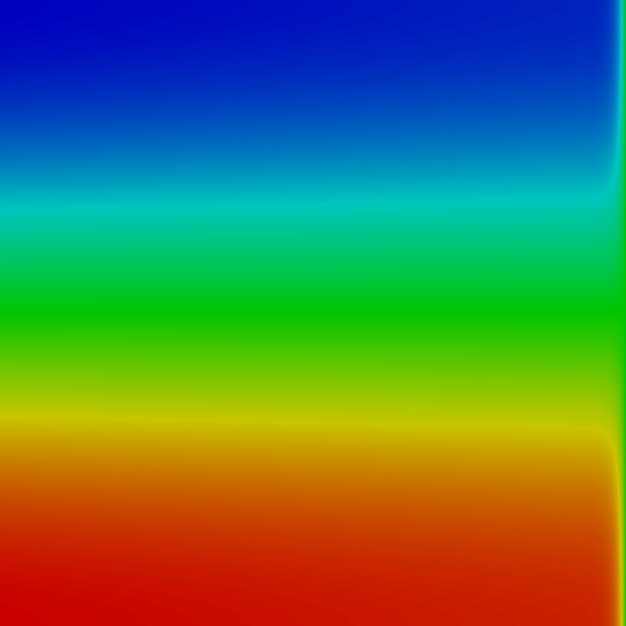
\includegraphics[width=0.6\textwidth]{figs/Erickson/exact.png}
\caption{Erickson-Johnson exact solution}
\label{fig:erickson}
\end{figure}

\begin{figure}[p]
\centering
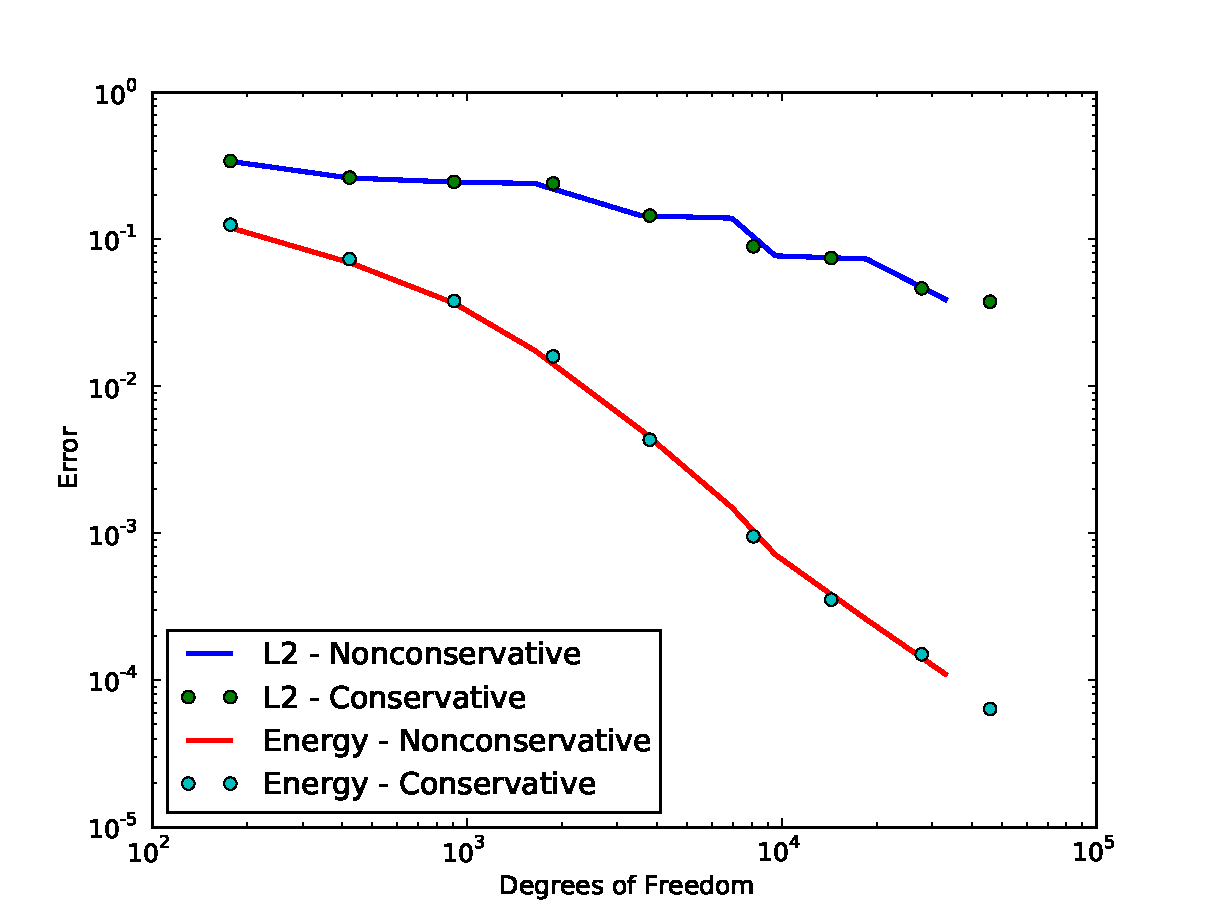
\includegraphics[width=0.8\textwidth]{figs/Erickson/modifiedError.pdf}
\caption{Error in Erickson-Johnson solutions}
\label{fig:ericksonError}
\end{figure}

\begin{figure}[h!]
\centering
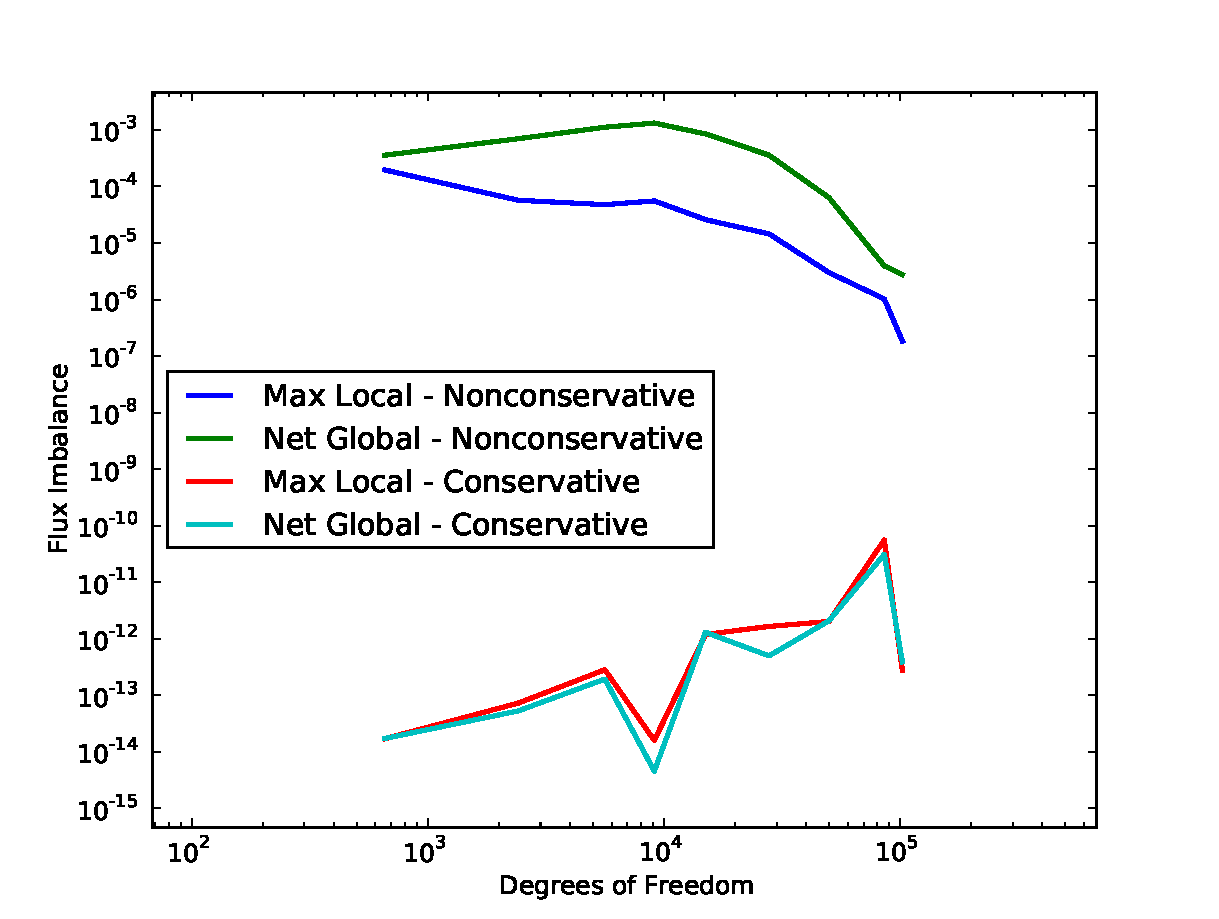
\includegraphics[width=0.8\textwidth]{figs/Erickson/graphFlux.pdf}
\caption{Flux imbalance in Erickson-Johnson solutions}
\label{ericksonFlux}
\end{figure}

\subsubsection{Skewed Convection-Diffusion Problem}
This is a standard convection-diffusion problem with a skewed convection
vector relative to the mesh. We take $\bbeta=(2,1)$, and on the left and
bottom inflow boundaries we impose $\hat t=1-x-y$ while the right and top
boundaries have $\hat u=0$. We solve for $\epsilon=10^{-4}$. 

\begin{figure}[p]
\centering
\begin{subfigure}[t]{0.45\textwidth}
\centering
\includegraphics[width=\textwidth]{figs/Confusion/modified8nc.png}
\includegraphics[width=\textwidth]{figs/Confusion/modified8nc_mesh.png}
\caption{Nonconservative}
\label{fig:confusionModified8nc}
\end{subfigure}
\begin{subfigure}[t]{0.45\textwidth}
\centering
\includegraphics[width=\textwidth]{figs/Confusion/modified8c.png}
\includegraphics[width=\textwidth]{figs/Confusion/modified8c_mesh.png}
\caption{Conservative}
\label{fig:confusionModified8c}
\end{subfigure}
\caption{Skewed convection-diffusion problem after 8 refinements}
\label{fig:confusion}
\end{figure}

\begin{figure}[h!]
\centering
\includegraphics[width=0.8\textwidth]{figs/Confusion/modifiedFlux.pdf}
\caption{Flux imbalance in skewed convection-diffusion solutions}
\label{fig:confusionFlux}
\end{figure}

\subsubsection{Double Glazing Problem}
This nominal problem definition takes the same unit square domain with 
\[
\bbeta=\binom{2(2y-1)(1-(2x-1)^2)}{-2(2x-1)(1-(2y-1)^2)}\,;\quad
\hat u=
\begin{cases}
1 & \mbox{on }\Gamma_{right}\\
0 & \mbox{else }
\end{cases}\,,
\]
except that this definition for the boundary is not legal for $\hat u\in
H^{\frac{1}{2}}(\Gamma_h)$ which is continuous. Therefore we use a ramp of
width $\sqrt{\epsilon}$ on the right edge to go from 0 to 1. The 
results are for $\epsilon=10^{-2}$.

\begin{figure}[p]
\centering
\begin{subfigure}[t]{0.45\textwidth}
\centering
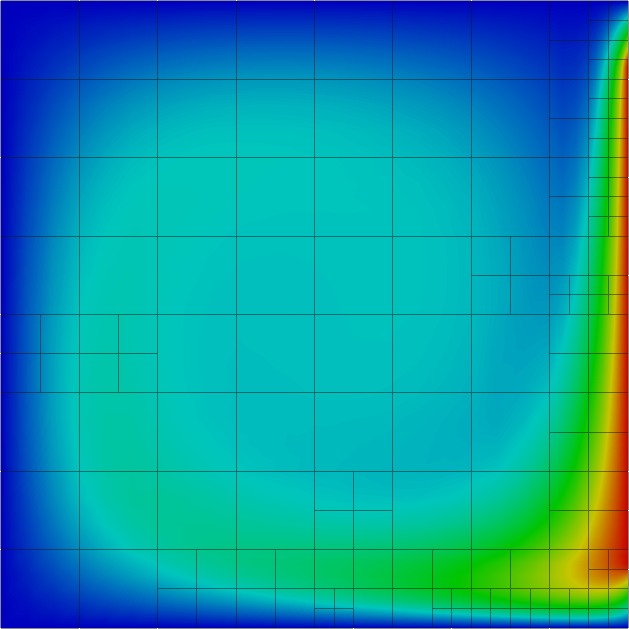
\includegraphics[width=\textwidth]{figs/DoubleGlazing/modified5nc.png}
\caption{Nonconservative}
\label{fig:doubleglazingGraph6c}
\end{subfigure}
\begin{subfigure}[t]{0.45\textwidth}
\centering
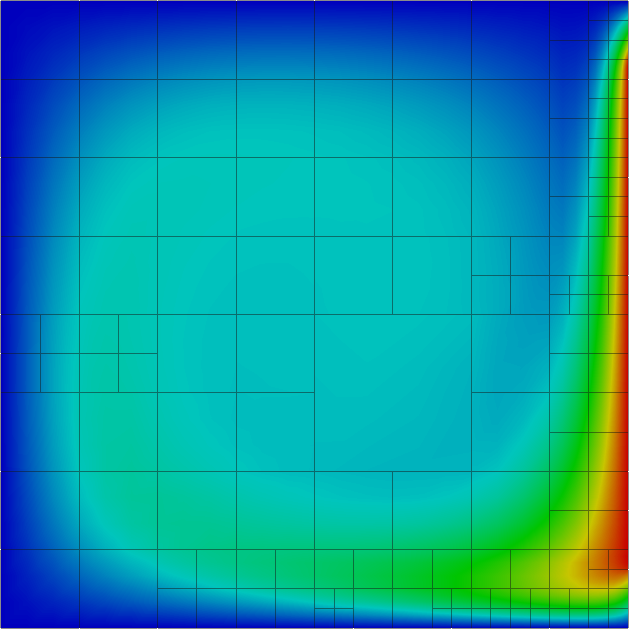
\includegraphics[width=\textwidth]{figs/DoubleGlazing/modified5c.png}
\caption{Conservative}
\label{fig:doubleglazingRobust6c}
\end{subfigure}
\caption{Double glazing problem after 5 refinements}
\label{fig:doubleglazing}
\end{figure}

\begin{figure}[p]
\centering
\includegraphics[width=0.8\textwidth]{figs/DoubleGlazing/modifiedFlux.pdf}
\caption{Flux imbalance in double glazing problem}
\label{fig:doubleglazingFlux}
\end{figure}

\subsubsection{Vortex Problem}
This problem models a mildly diffusive vortex convecting fluid in a circle. We
deal with domain $\Omega=[-1,1]^2$, with $\epsilon=10^{-4}$, and
$\bbeta=(-y,x)^T$. Note that $\bbeta=\mathbf{0}$ at the domain center. We have an
inflow boundary condition when $\bbeta\cdot\mathbf{n}<0$, in which case we set
$\hat t=\bbeta\cdot\mathbf{n}\cdot u_0$ where
$u_0=\frac{\sqrt{x^2+y^2}-1}{\sqrt{2}-1}$ which will vary from 0 at the center
of boundary edges to 1 at corners. We don't enforce an outflow boundary.

\begin{figure}[p]
\centering
\begin{subfigure}[t]{0.45\textwidth}
\centering
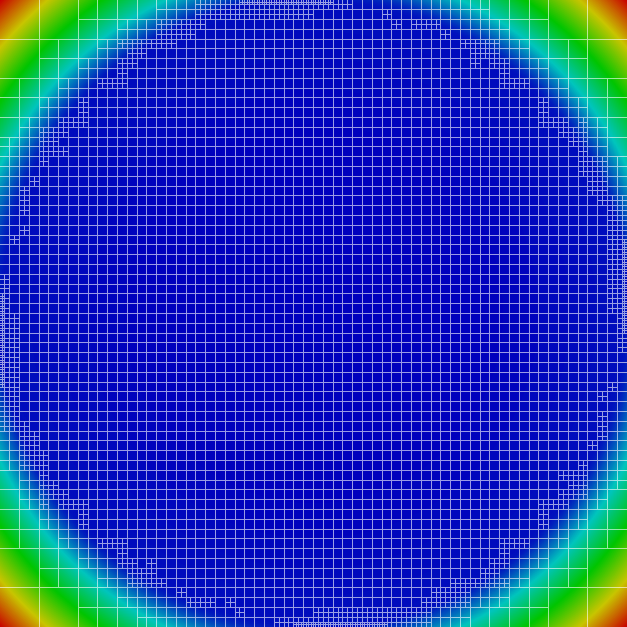
\includegraphics[width=\textwidth]{figs/Vortex/modified6nc.png}
\caption{Nonconservative}
\label{fig:vortexModified6nc}
\end{subfigure}
\begin{subfigure}[t]{0.45\textwidth}
\centering
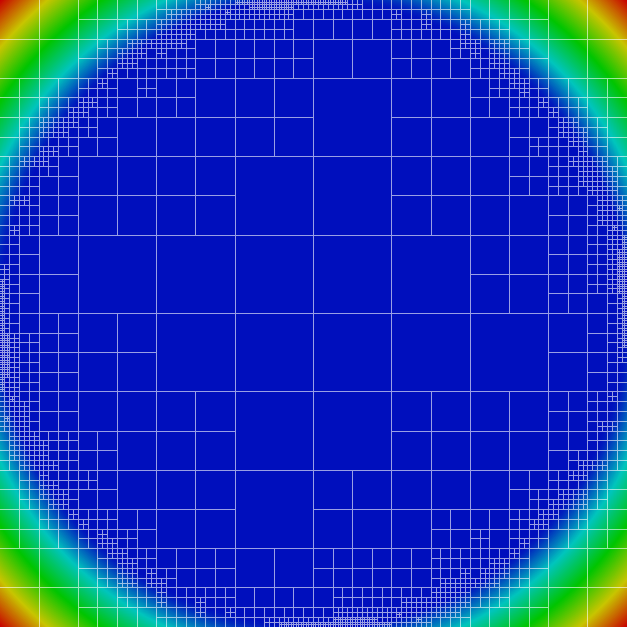
\includegraphics[width=\textwidth]{figs/Vortex/modified6c.png}
\caption{Conservative}
\label{fig:vortexModified6c}
\end{subfigure}
\caption{Vortex problem after 6 refinements}
\label{fig:vortex}
\end{figure}

\begin{figure}[p]
\centering
\includegraphics[width=0.8\textwidth]{figs/Vortex/modifiedFlux.pdf}
\caption{Flux imbalance in vortex solutions}
\label{fig:vortex_flux}
\end{figure}

\subsubsection{Wedge Problem}
We devised this problem to examine some of the issues we were having blow up
of the solution under the robust test norm. The domain is a rectangle
$[-0.5,0.5]\times[-1,0.5]$ where the triangle connecting the bottom edges with
the origin at $(0,0)$ is removed. The convection vector $\bbeta=(1,0)^T$,
$\epsilon=10^{-1}$, and we apply boundary conditions $\hat t=0$ on the left
inflow edge, $\hat u=0$ on the top edge, $\bbeta\cdot\mathbf{n}\cdot\hat
u-\hat t=\sigma_n=0$ on the right outflow edge, $\hat u=1$ on the leading edge
of the wedge, and $\hat t=\bbeta\cdot\mathbf{n}\cdot 1$ on the trailing edge
of the wedge.

\begin{figure}[p]
\centering
\begin{subfigure}[t]{0.4\textwidth}
\centering
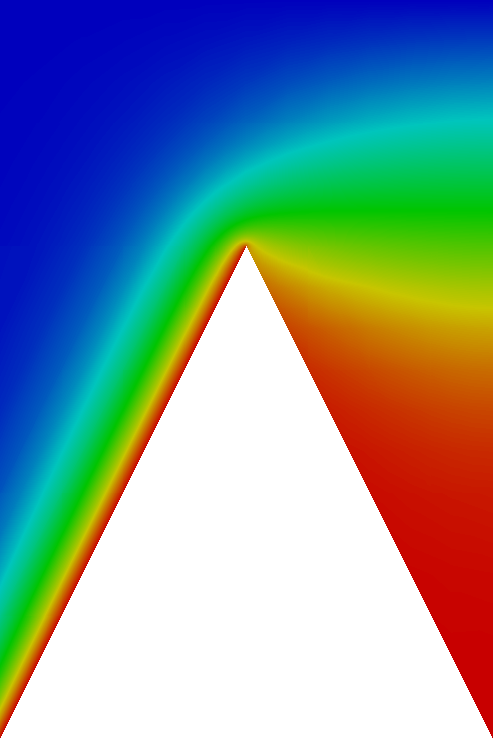
\includegraphics[width=\textwidth]{figs/Wedge/modified16nc.png}
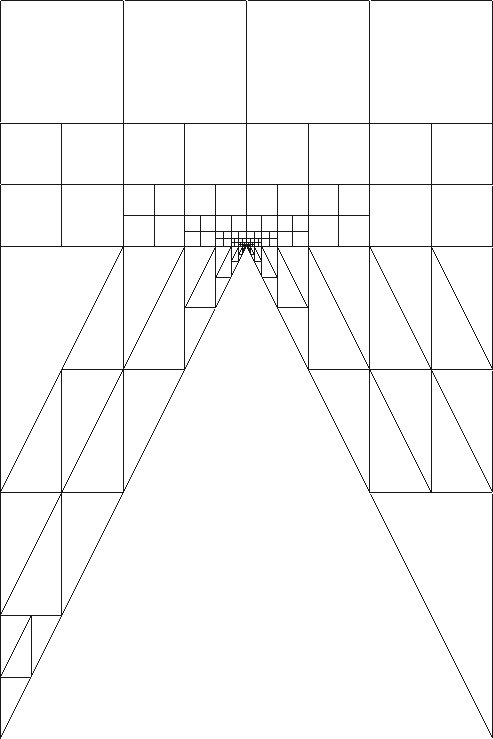
\includegraphics[width=\textwidth]{figs/Wedge/modified16nc_mesh.png}
\caption{Nonconservative}
\label{fig:wedgeGraph16nc}
\end{subfigure}
\begin{subfigure}[t]{0.4\textwidth}
\centering
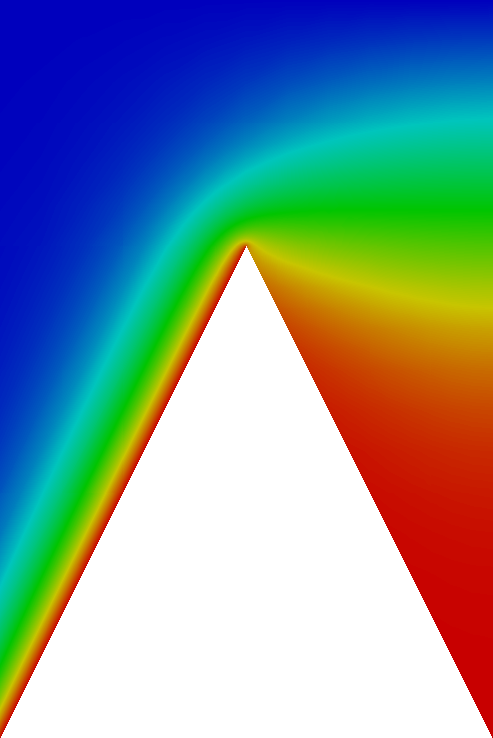
\includegraphics[width=\textwidth]{figs/Wedge/modified16c.png}
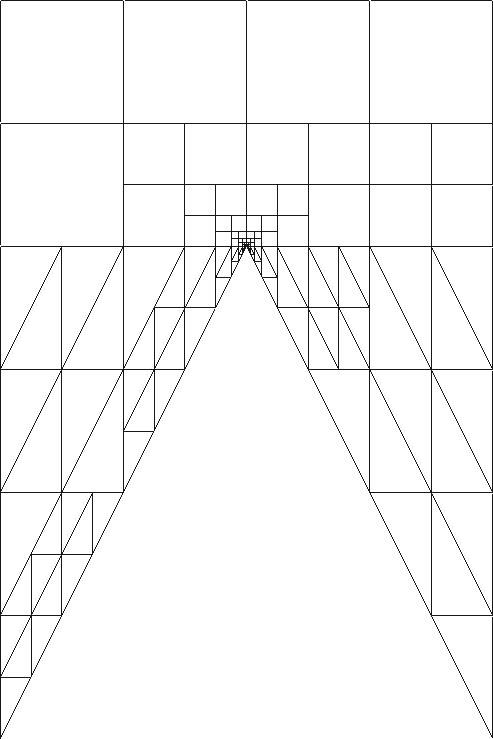
\includegraphics[width=\textwidth]{figs/Wedge/modified16c_mesh.png}
\caption{Conservative}
\label{fig:wedgeRobust16nc}
\end{subfigure}
\caption{Wedge problem after 16 refinements}
\label{fig:wedge}
\end{figure}

\begin{figure}[p]
\centering
\includegraphics[width=0.8\textwidth]{figs/Wedge/modifiedFlux.pdf}
\caption{Flux imbalance in wedge solutions}
\label{fig:wedge_flux}
\end{figure}

\subsubsection{Inner Layer Problem}
In this problem, $\bbeta=(\frac{\sqrt{3}}{2},\frac{1}{2})^T$ and we have a
discontinuous flux inflow condition where $\hat t=0$ if $y\le0.2$ and $\hat
t=\bbeta\cdot\mathbf{n}$ if $y>0.2$. On the outflow, $\hat u=0$. We use a very
small diffusion scale of $\epsilon=10^{-6}$ which creates a very thin inner
layer.
% Nonconservative solution in range $[-0.38, 1.34]$.
% Conservative solution in range $[-0.39, 1.38]$.

\begin{figure}[p]
\centering
\begin{subfigure}[t]{0.45\textwidth}
\centering
\includegraphics[width=\textwidth]{figs/InnerLayer/modified8nc.png}
\includegraphics[width=\textwidth]{figs/InnerLayer/modified8nc_mesh.png}
\caption{Nonconservative}
\label{fig:innerlayer8nc}
\end{subfigure}
\begin{subfigure}[t]{0.45\textwidth}
\centering
\includegraphics[width=\textwidth]{figs/InnerLayer/modified8c.png}
\includegraphics[width=\textwidth]{figs/InnerLayer/modified8c_mesh.png}
\caption{Conservative}
\label{fig:innerlayer8c}
\end{subfigure}
\caption{Inner layer problem after 8 refinements}
\label{fig:innerlayer}
\end{figure}

\begin{figure}[p]
\centering
\includegraphics[width=0.8\textwidth]{figs/InnerLayer/modifiedFlux.pdf}
\caption{Flux imbalance in inner layer solutions}
\label{fig:innerlayer_flux}
\end{figure}

\subsubsection{Discontinuous Source Problem}
Here, $\bbeta=(0.5,1)^T/\sqrt{1.25}$, and we have a discontinuous source term
such that $f=1$ when $y\ge2x$ and $f=-1$ when $y<2x$. We apply boundary
conditions of $\hat t=0$ on the inflow and $\hat u=0$ on the outflow. Contrary
to the other problems discussed, the solution for this problem does not range
from 0 to one. Rather, the colorbar in Figure \ref{fig:discontinuous} is
scaled to  $[-1.110,0.889]$.

\begin{figure}[p]
\centering
\begin{subfigure}[t]{0.45\textwidth}
\centering
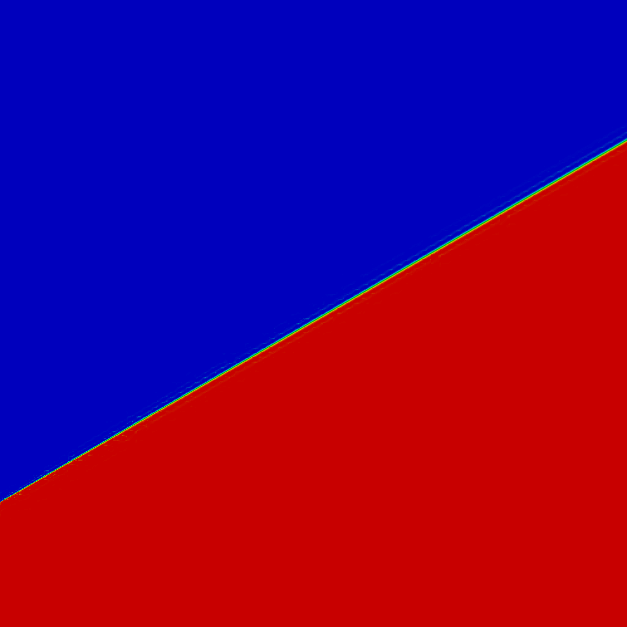
\includegraphics[width=\textwidth]{figs/Discontinuous/graph8nc.png}
\caption{Nonconservative}
\label{fig:discontinuousModified8nc}
\end{subfigure}
\begin{subfigure}[t]{0.45\textwidth}
\centering
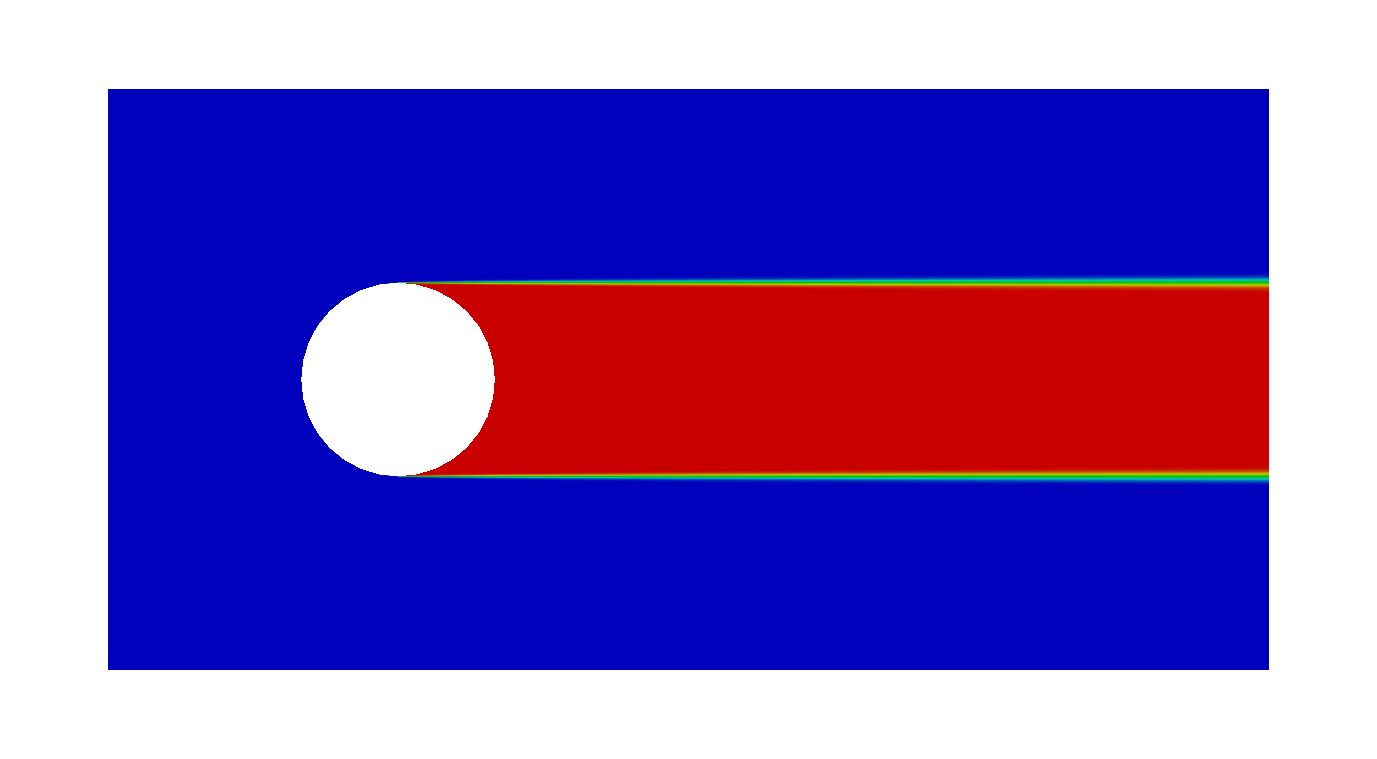
\includegraphics[width=\textwidth]{figs/Discontinuous/robust8nc.png}
\caption{Conservative}
\label{fig:discontinuousModified8c}
\end{subfigure}
\caption{Discontinuous source problem after 8 refinements}
\label{fig:discontinuous}
\end{figure}

\begin{figure}[p]
\centering
\includegraphics[width=0.8\textwidth]{figs/Discontinuous/modifiedFlux.pdf}
\caption{Flux imbalance in discontinuous source solutions}
\label{fig:discontinuous_flux}
\end{figure}

\subsubsection{Hemker Problem}
The Hemker problem is defined on a domain
$\Omega=\{[-3,9]\times[-3,3]\}\setminus\{(x,y):x^2+y^2<1\}$, essentially a simplified
model of flow past an infinite cylinder. We start with the initial mesh shown
in Figure~\ref{fig:hemkerInitial} in which we approximate the circle by 8
fourth order curvilinear polynomial segments. As we refine, the new elements are
fitted to better approximate an exact circle.The boundary conditions are $\hat
t=\bbeta\cdot\mathbf{n}\cdot 1$ on the left inflow boundary,
$\bbeta\cdot\mathbf{n}\cdot\hat u-\hat t=\sigma_n=0$ on the right outflow
boundary, $\hat t=0$ on the top and bottom edges, and $\hat u=1$ on the
cylinder.

\begin{figure}[p]
\centering
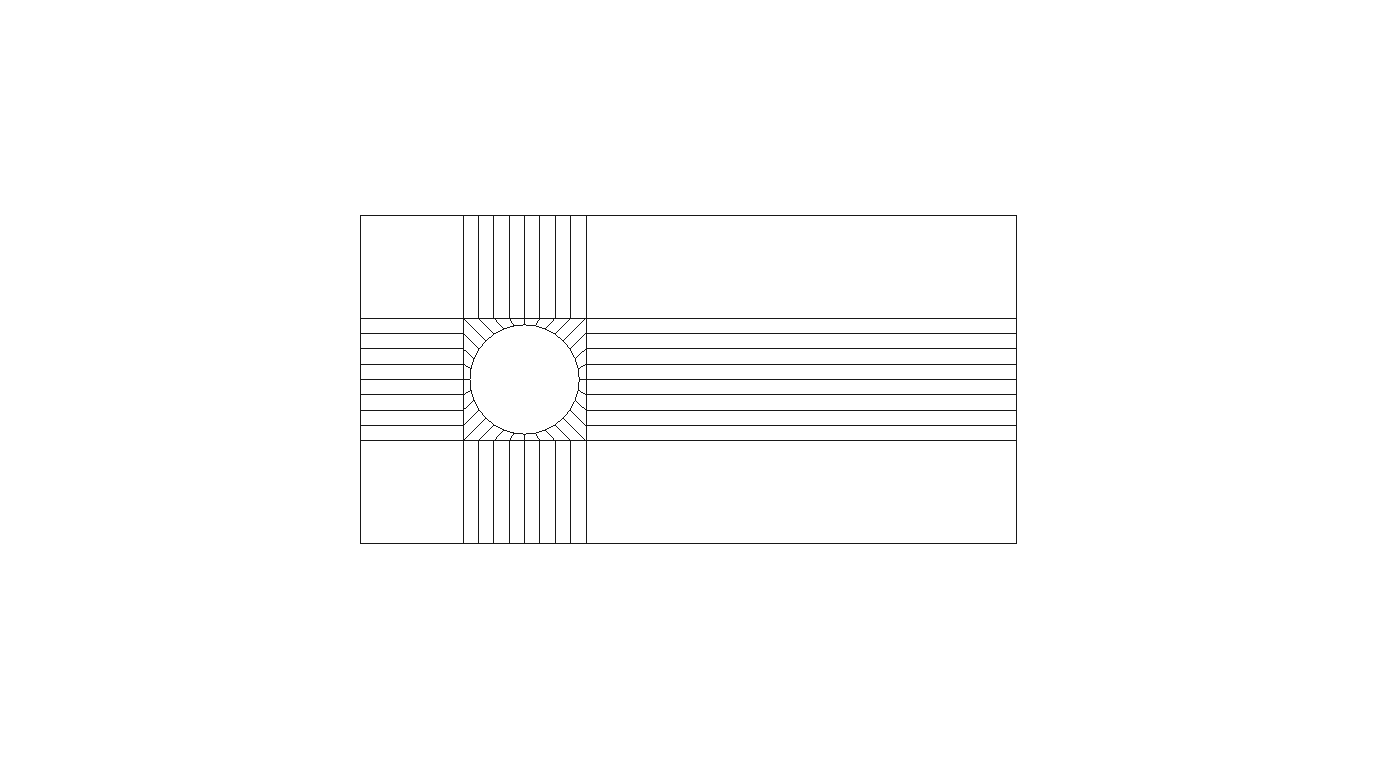
\includegraphics[width=0.8\textwidth]{figs/Hemker/initial_mesh.png}
\caption{Initial mesh for the Hemker problem}
\label{fig:hemkerInitial}
\end{figure}

\begin{figure}[p]
\centering
\begin{subfigure}[t]{0.6\textwidth}
\centering
\includegraphics[width=\textwidth]{figs/Hemker/modified8nc.png}
\end{subfigure}
\begin{subfigure}[t]{0.6\textwidth}
\centering
\includegraphics[width=\textwidth]{figs/Hemker/modified8nc_mesh.png}
\caption{Nonconservative}
\label{fig:hemkerModified8nc}
\end{subfigure}
\begin{subfigure}[t]{0.6\textwidth}
\centering
\includegraphics[width=\textwidth]{figs/Hemker/modified8c.png}
\end{subfigure}
\begin{subfigure}[t]{0.6\textwidth}
\centering
\includegraphics[width=\textwidth]{figs/Hemker/modified8c_mesh.png}
\caption{Conservative}
\label{fig:hemkerModified8c}
\end{subfigure}
\caption{Hemker problem after 8 refinements}
\label{fig:hemker8}
\end{figure}

\begin{figure}[p]
\centering
\centering
\includegraphics[width=0.8\textwidth]{figs/Hemker/modifiedFlux.pdf}
\caption{Flux imbalance in Hemker problem}
\label{fig:hemkerFlux}
\end{figure}

\subsection{Analysis of Results}\label{sec:problemAnalysis}
% Solution quality
The general trend we see looking at the results is that the solution quality
of the conservative and conconservative formulations is nearly identical. This
is ideal, as we wish to preserve the attractive features of DPG --
namely that it minimizes error in the energy norm. In particular, when we
examine the error convergence plots for the Erickson-Johnson problem, the
energy levels for the two methods lie nearly right on top of each other. This
seems to indicate at the least that enforcing local conservation doesn't hurt
DPG too much.

% Overshoots/undershoots
Another measure of solution quality is to look at the magnitude of overshoots
and undershoots in the solution. In most of the problems considered (barring
the discontinuous source problem) the exact solution would range exactly
between 0 and 1. The the resolved solutions, the divergence from these values
would be negligible, but for the inner layer, in which $\epsilon=10^{-6}$, we
get overshoots and undershoots along the separation line. For the
nonconservative formulation, the solution range for $u$ was $[-0.392,1.342]$,
while the conservative solution range was $[0.389,1.378]$. This difference is
easily accounted for by the differences in refinement patterns between the two
methods.

% Mesh refinements
It is clear when comparing the refinement patterns that the two methods appear
to calculate slightly different error representation functions (which
determine which elements to adaptively refine). Standard DPG minimizes the
error in the energy norm, but the Lagrange multipliers in the conservative
formulation shift the solution slightly. So we should see somewhat higher
error and different elements will get chosen for refinement. The choice of
test norm also plays into this calculation of the error representation
function. As discussed earlier, the conservative formulation allows us to
throw away the $L^2$ term on $v$. The inclusion of this term required certain
assumptions on $\bbeta$ \cite{ChanHeuerThanhDemkowicz2012} that break down for
the vortex problem. Here we see the nonconservative method needlessly refine
in the center of the domain where the solution is constant. The conservative
scheme is more discerning about refinements and focuses refinements where
solution features are changing. In general, though, both methods appear to
follow very similar refinement patterns.

% Mass conservation
It shouldn't come as a surprise that the conservative and nonconservative
solutions match each other so closely. The conservative formulation
enforces local conservation more strictly, but if we examine the flux
imbalance plots, the nonconservative formulation is nearly conservative on its
own -- and appears to become more conservative with refinement. The flux
imbalance of the conservative methods appears to bounce around close to the
machine epsilon (plus a few orders of magnitude). The level of enforcement
appears to creep up with more degrees of freedom, indicating possible
accruement of numerical error.


\section{A coupled, robust test norm}
In the course of our numerical experiments, we encountered unforseen
difficulties for certain problems under our current robust test norm.  We
illustrate in this section the observed issue using a second model problem
with a singular solution, offer possible explanations for the phenomena
observed, and propose a modification of the robust test norm presented
previously, which we demonstrate eliminates the issues observed in numerical
experiments.  


\subsection{A second model problem}
\seclab{sec:confusionPlate}
We begin by first examining a different problem than convection-diffusion --
we examine admissible solutions for the homogeneous Laplace's equation over
the $y > 0$ half-plane under boundary conditions 
\begin{align*}
u &= 0 \text{ on } x > 0\\
\pd{u}{n} &= 0 \text{ on } x < 0.
\end{align*}
Let us consider the 2D case - a simple separation of variables argument in
polar coordinates shows that the solution is of the form
\[
u(r,\theta) = \sum_{n=0}^\infty R_n(r) \sin(\lambda_n \theta),
\]
where $\lambda_n = n + \frac{1}{2}$, and $R_n(r) = C_{1,n}x^{\lambda_n} + C_{2,n}x^{-\lambda_n}$.  By requiring $u(0,\theta) < \infty$, we have $R_n(r) = C_n x^{\lambda_n}$.  We have now that solutions to this problem include $u$ of the form
\[
u = \sum_{n=0} x^{n+\frac{1}{2}} \sin\LRp{\LRp{n+\frac{1}{2}}\theta}.
\]
Note that even in the lowest-order term, the gradient of $u$ displays a
singularity at $r = 0$.  \textcolor{red}{Find reference in that solutions to
Laplace's equation always can be split into smooth and singular parts on
similar domains.}  

Consider now Laplace's equation $\del u = f$ on the box domain $\Omega =
[0,1]^2$ with boundary conditions
\begin{align*}
u &= 0 \text{ on } x > .5\\
\pd{u}{n} &= 0 \text{ on } x < .5.
\end{align*}
with forcing term $f=1$.  
\begin{figure}[!h]
\centering
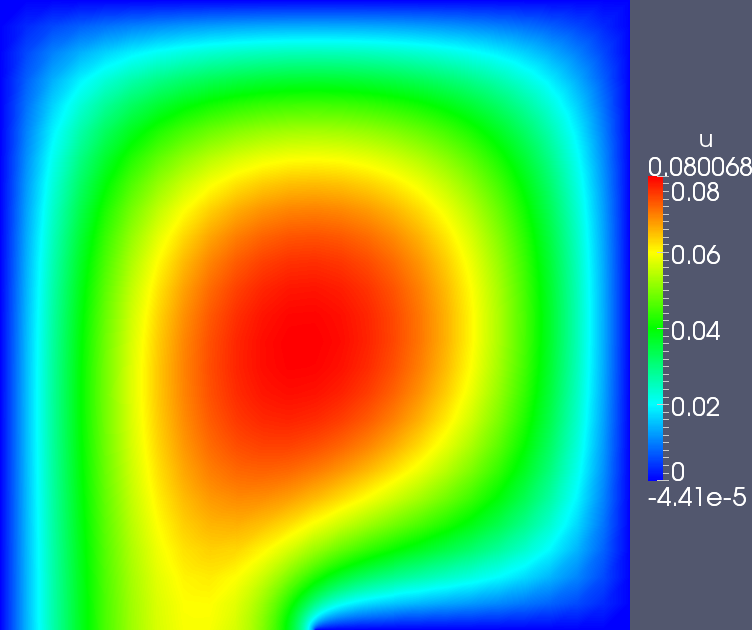
\includegraphics[scale=.375]{figs/LaplaceFigs/LaplacePlate.png}
\caption{Solution of Laplace's equation on the unit quad with $f=1$.}
\label{fig:laplace}
\end{figure}
Extrapolating the results from the half-plane example to a finite domain, we
expect the solution of Laplace's equation to be bounded, but to have a
singularity in its gradient.  Figures~\ref{fig:laplace} and
\ref{fig:laplaceStresses} are finite element solutions of the above problem
under a quadratic $h$-refined mesh.  Figure~\ref{fig:laplace} confirms that
$u$ is bounded, while Figure~\ref{fig:laplaceStresses} confirms that
singularities in the gradient appear at the point $(.5,0)$, where the boundary
condition changes from Neumann to Dirichlet.  

\begin{figure}[!h]
\centering
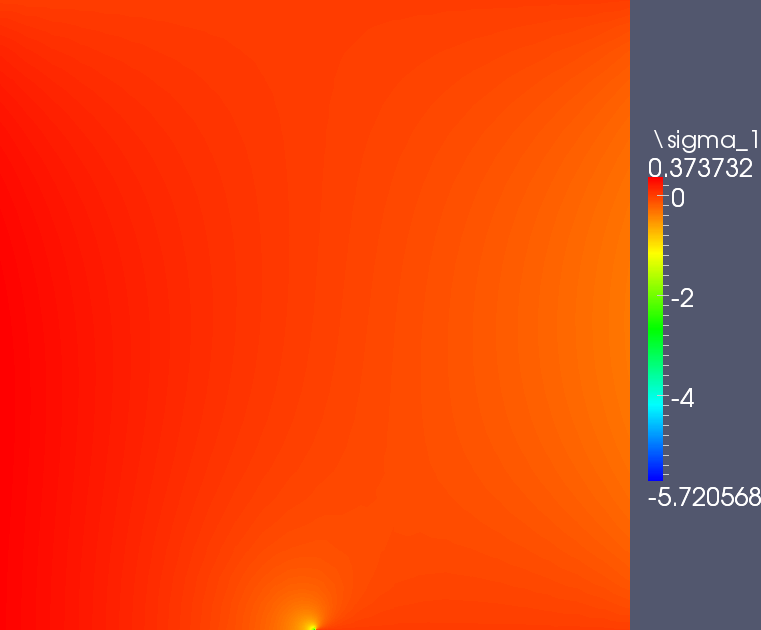
\includegraphics[scale=.275]{figs/LaplaceFigs/LaplacePlateSigma1.png}
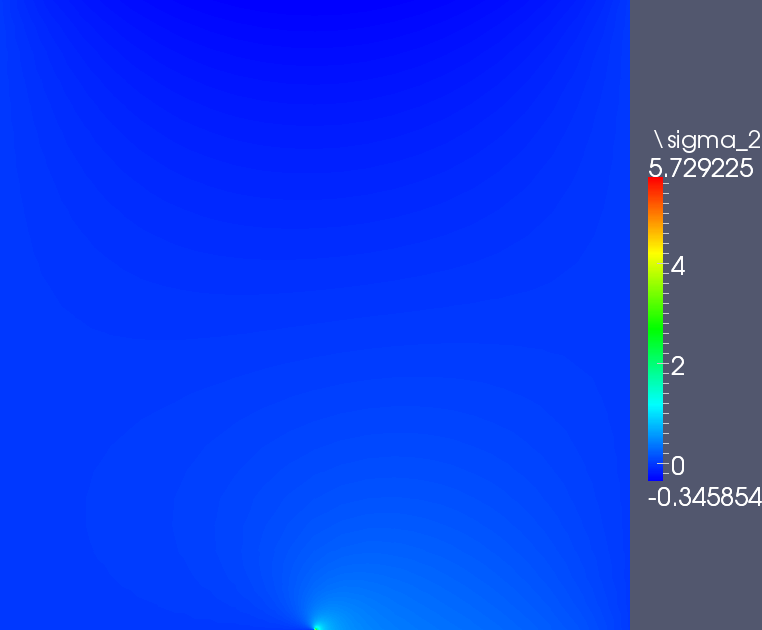
\includegraphics[scale=.275]{figs/LaplaceFigs/LaplacePlateSigma2.png}
\caption{$x$ and $y$ components of the $\Grad u$ for $u$ solving Laplace's equation with a change in boundary conditions.  Both components develop singularities at the point where the boundary condition changes type.}
\label{fig:laplaceStresses}
\end{figure}

We consider now the convection-diffusion problem, under a similar setup as
before.  We consider the domain $\Omega = [0,1]^2$, with boundary conditions
\begin{align*}
u &= 0,\quad \text{ on } x = 0\\
\pd{u}{n} &= 0,\quad \text{ on } x = 1, y = 1, \text{ and } y = 0, x < .5\\
u &= 1,\quad \text{ on } .5 < x \leq 1.
\end{align*}
The problem is meant to simulate the transport of $u$ over a domain with a
``plate'' boundary $x \in [.5,1]$.  For small $\epsilon$, the problem develops
a boundary layer over the plate, as well as a singularity at the plate tip
$(x,y) = (.5,0)$.\footnote{This problem is meant to mimic the Carter flat
plate problem -- a common early benchmark problem in viscous compressible flow
problems -- which can be shown to also exhibit a singularity in stress at the
point $(.5,0)$.}  Unlike the Laplace example, we swap the Dirichlet boundary
condition at the outflow $x=1$ with an outflow boundary
condition.\footnote{The outflow ``boundary condition'' is simply the absence
of an applied boundary condition, and is analyzed in more detail in
\cite{FLD:FLD505}.  This outflow condition appears to work well for
convection-diffusion problems in the convective regime, and is the outflow
condition we will use in our extension of DPG to a model problem in viscous
compressible flow.  Though the well-posedness of the problem under this
boundary condition is questionable, we can still effectively illustrate the
issues present under the robust test norm using this problem setup.  }

The above convection-diffusion problem is related back to the earlier
Laplace/diffusion problem with a singularity -- in most of the domain,
convective effects dominate; however, if we  localizing the behavior of
Laplace's equation to a circle of $\epsilon$ around $(.5,0)$, then we again
see a discontinuity in the stresses.  Asymptotic expansion techniques indicate
that singularities in solutions are determined primarily by the highest order
differential operator present in the equation -- in other words, the addition
of a convective term to a scaled Laplacian (to recover the
convection-diffusion equation) will not alter the presence of a singularity in
the solution \cite{roos2008robust}.  

\begin{figure}[!h]
\centering
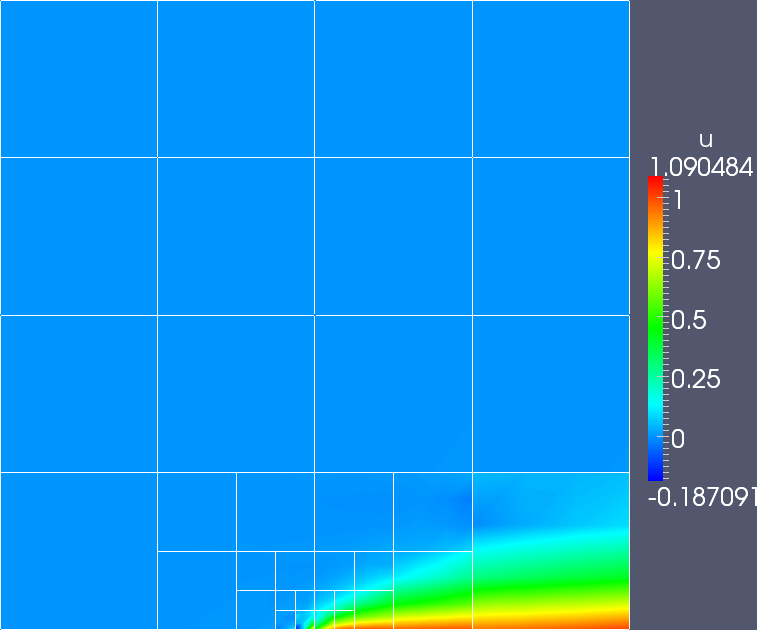
\includegraphics[scale=.275]{figs/LaplaceFigs/confusion1e2h1e2.png}
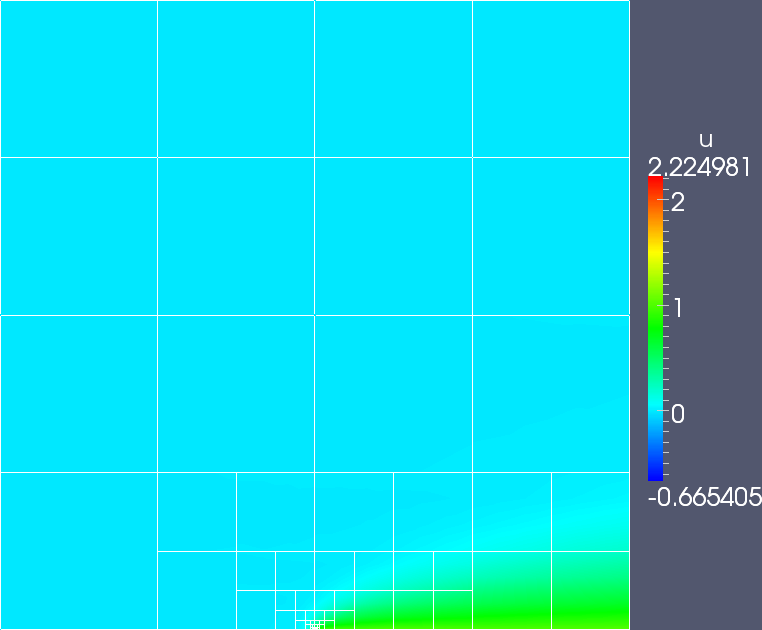
\includegraphics[scale=.275]{figs/LaplaceFigs/confusion1e2h1e3.png}
\caption{Solution $u$ for $\epsilon = .01$ under the robust test norm.  The solution oscillates strongly at the plate edge, growing in magnitude under additional refinements despite the absence of a singularity in $u$ at that point.}
\label{fig:plateOsc}
\end{figure}

Figures~\ref{fig:plateOsc} and \ref{fig:plateOscZoom} demonstrate the behavior
of the DPG method under the robust test norm for the plate problem.  The
diffusion is taken to be fairly large ($\epsilon = 10^{-2}$), and automatic
refinements are done until the element size $h$ is at or below the diffusion
scale.  Due to the singular nature of the solution, refinements are clustered
around $(.5,0)$, and the order is set to be uniform with $p=2$.  While there
should be no singularity in $u$, the magnitude of $u$ grows as $h \rightarrow
0$, so long as $h\leq \epsilon$.  

\begin{figure}[!h]
\centering
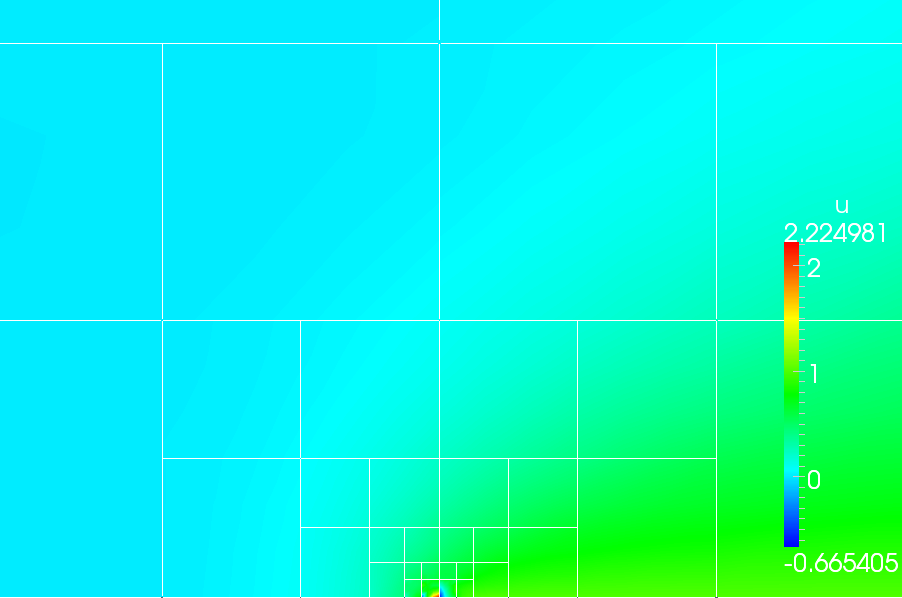
\includegraphics[scale=.375]{figs/LaplaceFigs/confusion1e2h1e3uZoom.png}
\caption{Zoomed solution $u$ and adaptive mesh for $\epsilon = .01$ after over-resolution of the diffusion scale. }
\label{fig:plateOscZoom}
\end{figure}

We note that the appearance of this non-physical singularity in $u$ is allowed
under the theory underlying the robust test norm; the error in the $\L$-norm
of the solution is guaranteed to be robustly bounded; however, the $\L$ norm
does allow for the presence of weak singularities (singularities of order
$x^{-\frac{1}{2}}$).  Apart from the oscillation of $u$ at the singular point,
the solution is well-behaved, and the stress $\sigma = \epsilon \Grad u$ is
very well represented, as indicated in Figure~\ref{fig:plateStresses}.  

\begin{figure}[!h]
\centering
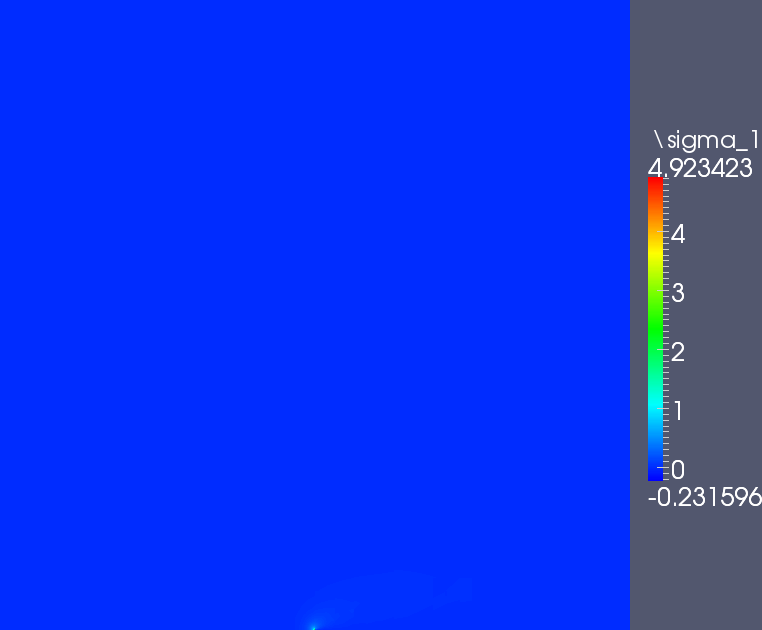
\includegraphics[scale=.275]{figs/LaplaceFigs/confusion1e2h1e3Sigma1.png}
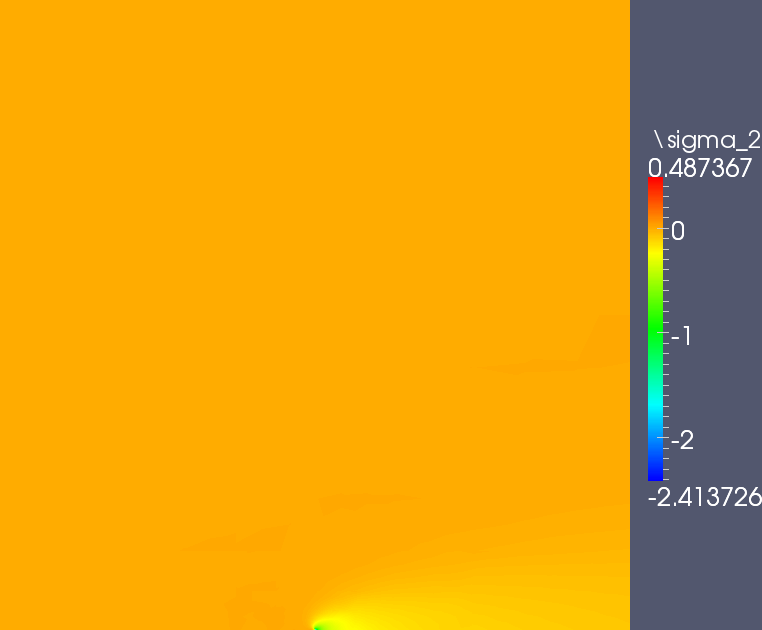
\includegraphics[scale=.275]{figs/LaplaceFigs/confusion1e2h1e3Sigma2.png}
\caption{Viscous stresses for the plate problem.  }
\label{fig:plateStresses}
\end{figure}

\subsection{A modification of the robust test norm}

While oscillations of this sort in a solution near a singular point may be
acceptable in certain simulations, it is a large problem for the methods in
compressible flow simulations -- physical constraints require several solution
variables to remain positive throughout simulation.\footnote{Apart from
returning a non-physical solution, the violation of positivity constraints
typically results in non-convergence of nonlinear solvers.}  We propose a
modification of the robust test norm that appears to remedy this issue, which
we refer to as 
\[
\norm{\LRp{v,\tau}}_V^2 \coloneqq \norm{v}^2_{\L} + \norm{\beta\cdot \Grad v}_{\L}^2 + \norm{\div \tau - \beta\cdot\Grad v}_{\L}^2 + \norm{C_\tau\tau}_{\L}^2,
\]
where $C_\tau$ is defined as before.
\footnote{
We note that we have dropped the
mesh-dependent scaling on $\norm{v}_{\L}$ from the robust norm; this is related
to recent insights into the nature of DPG test spaces and explained in more
detail in %Appendix~\secref{appendix:globalLocal}.
}  
We note that, under the
theory developed in 
% Section~\secref{sec:testNormSec}, 
the above test norm is
trivially provably robust using the same theory.
\footnote{This is due to the
fact that $\norm{\div \tau - \beta\cdot\Grad v}_{\L}^2$ is robustly bounded by
$\norm{\div \tau}_{\L}$ and $\norm{\beta\cdot\Grad v}_{\L}$.  Alternatively, we
can note that $\norm{\div \tau - \beta\cdot\Grad v}_{\L}^2 = \norm{g}_{\L}^2$,
where $g$ is a load of the adjoint problem related to robustness described in
% Section~\secref{sec:testNormSec}.
}

While not rigorously understood, the author believes the issues related to the
appearance of non-physical singularities to be related to the uncoupled nature
of the test norm.  Previous example problems exhibited boundary layers and
sharp gradients in the stress $\sigma$, but not singularities, which
contribute significantly more error.  We expect that the oscillations observed
in $u$ are a sort of \textit{pollution error}, where error in $u$ is tied to
error in $\sigma$.  If we consider the ultra-weak variational formulation for
convection-diffusion
\[
\LRp{u,\div \tau - \beta\cdot \grad v}_{\L} + \LRp{\sigma,\frac{1}{\epsilon} \tau + \grad v}_{\L} + \ldots,
\]
we can see that it is a combination of test functions that corresponds to both
$u$ and $\sigma$.  Recall from the previous section that, by choosing $\tau$
and $v$ such that they satisfy the adjoint equation with forcing terms $u$ and
$\sigma$, we recover the best $L^2$ approximation.  In other words, achieving
optimality in the $L^2$ norm requires coupling between $v$ and $\tau$, which
is achieved under the graph norm, but not the robust norm derived in the
previous section.  If coupling of the test terms , we expect that decoupling
$v$ and $\tau$ from each other in a test norm from each other will have the
effect of coupling error in $\sigma$ to error in $u$, which would explain the
spurious oscillations in $u$ in the presence of singularities in $\sigma$.
Similar results have been observed in the Stokes equations, where error in $u$
is coupled to the behavior of the pressure variable \cite{FLD:FLD582}.  

The drawback to using the above test norm is that the resulting local system
for test functions is now completely coupled, whereas using the previous test
norm, the system was block diagonal due to the decoupling in $v$ and $\tau$
and could be constructed and inverted more efficiently.  We hope to explore
the difference between these two norms in more rigor and detail in the
future.  

\begin{figure}[!h]
\centering
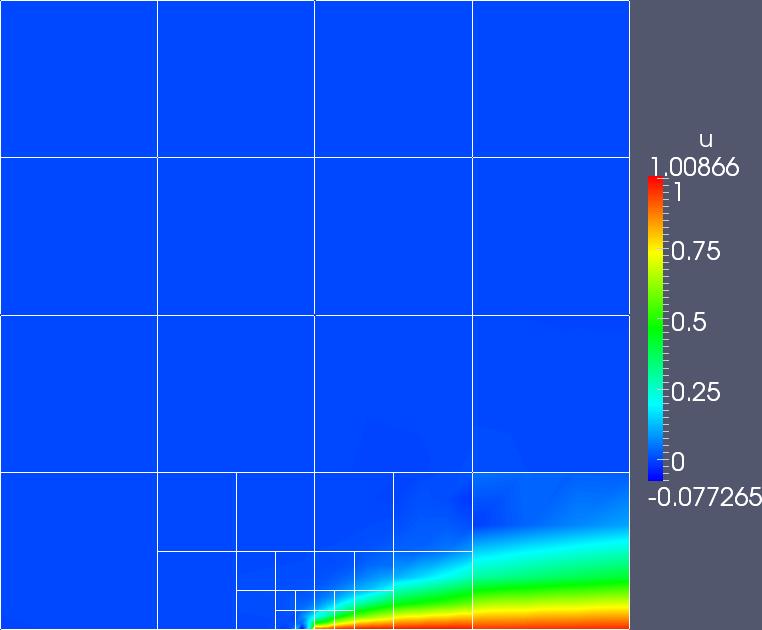
\includegraphics[scale=.275]{figs/LaplaceFigs/coupled1e2h1e2.png}
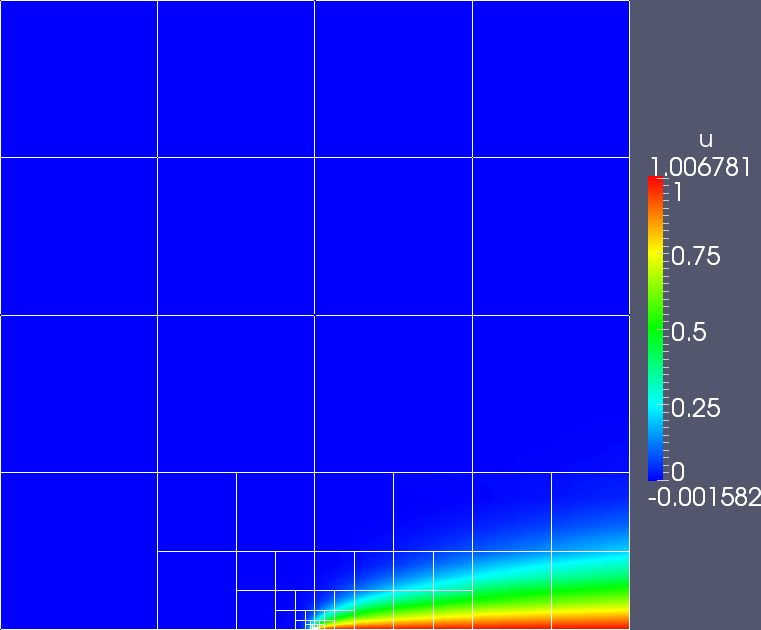
\includegraphics[scale=.275]{figs/LaplaceFigs/coupled1e2h1e3.png}
\caption{$\epsilon = 10^{-2}$ without $h$-resolving diffusion scale, and with $h$-resolution of diffusion scale.}
\label{fig:newNorm}
\end{figure}

Figure~\ref{fig:newNorm} shows the solution for $\epsilon = .01$, where the
diffusion scale is both underresolved and resolved by $h$-adaptivity.  In both
cases, there are no additional oscillations near the plate tip --
Figure~\ref{fig:newNormZoom} shows a zoomed image of the solution $u$ at the
point $(.5,0)$.  The stress is resolved similarly to the previous case;
however, the solution $u$ does not display spurious oscillations in either the
underresolved or resolved cases.  Figure~\ref{fig:newNormSmallEps} displays
the same quantities, but for $\epsilon = 10^{-4}$, in order to demonstrate
that the new test norm removes spurious oscillations in $u$ (in the presence
of singularities in $\sigma$) independently of $\epsilon$.  

\begin{figure}[!h]
\centering
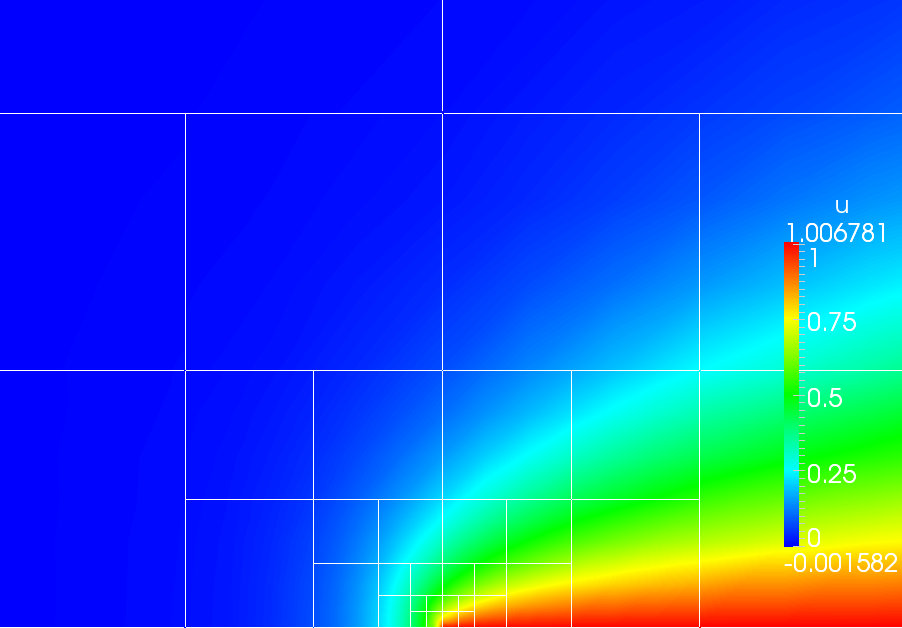
\includegraphics[scale=.3]{figs/LaplaceFigs/coupled1e2h1e3uZoom.png}
\caption{Zoom of solution $u$ at the plate tip for $\epsilon = 10^{-2}$.}
\label{fig:newNormZoom}
\end{figure}

\begin{figure}[!h]
\centering
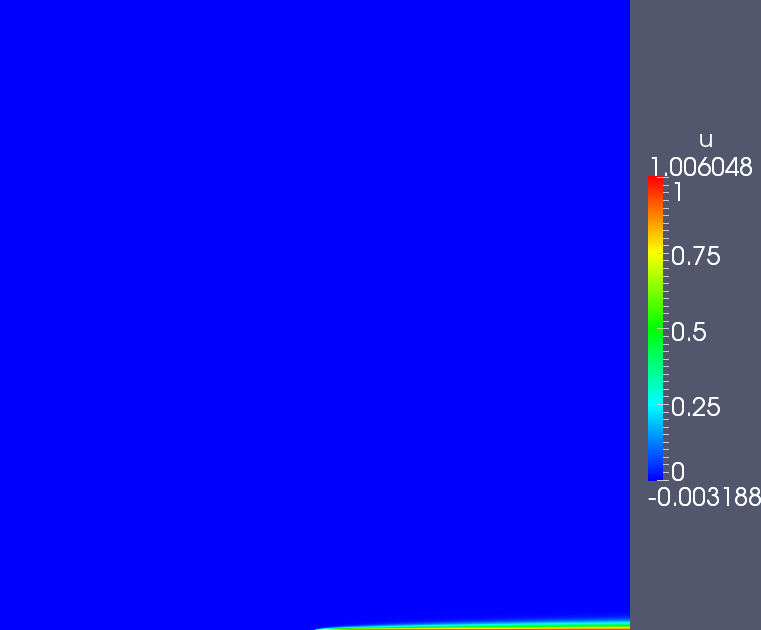
\includegraphics[scale=.25]{figs/LaplaceFigs/coupled1e4h1e5.png}
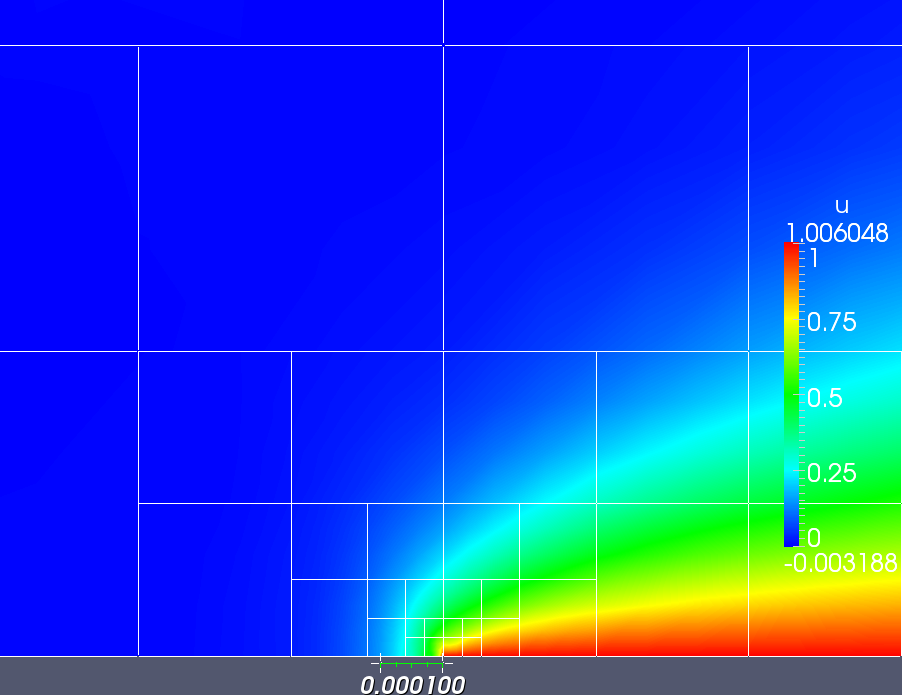
\includegraphics[scale=.227]{figs/LaplaceFigs/coupled1e4h1e5Zoom.png}
\caption{14 refinements for $\epsilon = 10^{-4}$, min $h$ is $O(10^{-5})$.}
\label{fig:newNormSmallEps}
\end{figure}

\bibliographystyle{plain} 
\bibliography{../../DPG} 
\end{document}

